\documentclass[a4paper,12pt,openany,oneside,utf-8]{ctexbook}
%\documentclass[a4paper,12pt,openany,oneside,utf-8]{cctbook}
%\usepackage{hyperref}
%\hypersetup{CJKbookmarks=true}
\usepackage{amssymb,amsmath}
\usepackage{subcaption}
\usepackage[amsmath,thmmarks]{ntheorem}
\usepackage{fancyhdr}

\usepackage{titletoc}%自己添加,
\usepackage{epsfig,picinpar}
\usepackage{setspace}
%\usepackage[top=2.54cm,bottom=2.54cm,left=2.54cm,right=2.54cm]{geometry}
\usepackage{geometry}
\geometry{left=3cm,right=2cm,top=2.5cm,bottom=2.5cm,}
\usepackage{amsmath}
\usepackage{mathtools} % offer \coloneqq to show := [see https://tex.stackexchange.com/questions/194344/symbol-for-definition]
%%%%%%%%%%%%%%%%%%%%%%%%new
\usepackage[super,square,comma,sort&compress]{natbib}
\usepackage{multirow}
\usepackage{dsfont}
\usepackage{booktabs}
\usepackage{epstopdf}
\bibliographystyle{gbt7714-2015}%{elsarticle-num}%{elsarticle-num}%{plain}%{elsarticle-num-names}%




%%%%%%%%%%%%%%%%%%%%%%自己的导言区
%\usepackage{natbib}     % adding a package for \citet{}, \citep{}, \citet*{}, \citep*{}
\usepackage{amssymb} %% The amssymb package provides various useful mathematical symbols
\newtheorem{theorem}{Theorem}[chapter]
\newtheorem{Definition}{Definition}[chapter]
\newtheorem{lemma}{Lemma}[chapter]
\newtheorem{proof}{Proof}[section]
\DeclareMathOperator*{\argmax}{arg\,max}
\usepackage{bm}         % adding a package for \bm{\widehat{\beta}}
\usepackage{makecell}   % makecell, see: https://blog.csdn.net/cy_tec/article/details/51436434
\usepackage{multirow}   % Latex Table, see: https://blog.csdn.net/canhui_wang/article/details/72920963
\usepackage{booktabs}   % for \cmidrule, see: https://zhidao.baidu.com/question/306414034088577164.html
\usepackage{graphicx}   % adding a package for loading figures
\usepackage{pdfpages}    % 加载PDF文件
\usepackage{threeparttable}   % adding a package for tablenotes
\usepackage{algorithm}
\usepackage{algorithmicx}
\usepackage{algpseudocode}
\usepackage{caption} %标题大小
\captionsetup{font={small}}

\usepackage{titlesec}    % for \titleformat
\usepackage{indentfirst}   % 关于首个段落缩进的问题, 可以在导言区加入宏包\usepackage{indentfirst}会自动缩进,  see: https://zhidao.baidu.com/question/207438548.html
\usepackage{caption}   % for \captionsetup, see: https://blog.csdn.net/kebu12345678/article/details/76957377?locationNum=9&fps=1
\usepackage{makecell}  % for \Xcline  \Xhline, see: http://blog.sina.com.cn/s/blog_5e16f1770100mvtd.html
\floatname{algorithm}{Algorithm}  % Ref: https://blog.csdn.net/lwb102063/article/details/53046265
\renewcommand{\algorithmicrequire}{\textbf{Input:}}
\renewcommand{\algorithmicensure}{\textbf{Output:}}
\usepackage{paralist} % for \begin{enumerate}, see: http://bbs.ctex.org/forum.php?mod=viewthread&tid=62084
%%%%%%%%%%%%%%%%%%%%%%自己的导言区



%%%%%%%%%%%%%%%%%%%%%%%%
%\renewcommand\sectionname{\arabic{section}}
%\renewcommand\sectionformat{\centering}
%\renewcommand\subsectionname{\arabic{section}.\arabic{subsection}}
%\renewcommand\subsectionformat{}
%\renewcommand\subsubsectionname{\arabic{section}.\arabic{subsection}.\arabic{subsubsection}}
%\renewcommand\subsubsectionformat{}

\allowdisplaybreaks[4]
\renewcommand{\baselinestretch}{1.5}
%\renewcommand{\chaptername}{{Chapter\thechapter}}
\renewcommand{\chaptername}{第{\thechapter}章}
\renewcommand\bibname{参考文献}
\renewcommand\contentsname{目录}
%\renewcommand{\sectionname}{{\thechapter}.\arabic{section}}

\renewcommand {\thetable} {\thechapter{}.\arabic{table}}
\renewcommand {\thefigure} {\thechapter{}.\arabic{figure}}
\renewcommand {\theequation} {\thechapter{}-\arabic{equation}}

% 字体大小设置
\newcommand{\chuhao}{\fontsize{48pt}{\baselineskip}\selectfont}
\newcommand{\xiaochuhao}{\fontsize{36pt}{\baselineskip}\selectfont}
\newcommand{\yihao}{\fontsize{28pt}{\baselineskip}\selectfont}
\newcommand{\xiaoyihao}{\fontsize{25pt}{\baselineskip}\selectfont}
\newcommand{\erhao}{\fontsize{21pt}{\baselineskip}\selectfont}
\newcommand{\xiaoerhao}{\fontsize{17pt}{\baselineskip}\selectfont}
\newcommand{\sanhao}{\fontsize{15.75pt}{\baselineskip}\selectfont}
\newcommand{\xiaosanhao}{\fontsize{15pt}{\baselineskip}\selectfont}
\newcommand{\sihao}{\fontsize{13pt}{\baselineskip}\selectfont}
\newcommand{\xiaosihao}{\fontsize{12pt}{\baselineskip}\selectfont}
\newcommand{\wuhao}{\fontsize{10.5pt}{\baselineskip}\selectfont}
\newcommand{\xiaowuhao}{\fontsize{9pt}{\baselineskip}\selectfont}
\newcommand{\liuhao}{\fontsize{7.875pt}{\baselineskip}\selectfont}
\newcommand{\qihao}{\fontsize{5.25pt}{\baselineskip}\selectfont}%\newcommand\kaishu{\CJKfamily{kai}}


\CTEXsetup[name={第,章}, number=\arabic{chapter}]{chapter}
\titleformat{\chapter}{\centering\sanhao\bfseries}{第\,\thechapter\,章}{1em}{}
\titlespacing*{\chapter} {0pt}{-10.5pt}{12pt}

\titleformat{\section}{\xiaosanhao\bfseries}{\thesection}{1em}{}
\titlespacing*{\section} {0pt}{12pt}{12pt}

\titleformat{\subsection}{\sihao\bfseries}{\thesubsection}{1em}{}
\titlespacing*{\subsection} {0pt}{0pt}{5.25pt}

\DeclareCaptionFont{fivehao}{\fontsize{10.5pt}{11pt}\selectfont #1}
\pagestyle{fancy}%
\renewcommand{\headrulewidth}{0pt}
\renewcommand{\footrulewidth}{0pt}
\addtolength{\headheight}{0\baselineskip}
\addtolength{\headwidth}{0\marginparsep}
\addtolength{\headwidth}{0\marginparwidth}
\setlength{\headsep}{5mm}%
\fancyhf{}


\begin{document}
	
	%
\includepdf{cover.pdf}
	\theoremstyle{plain} \theoremseparator{}
	\theoremindent0cm\theoremnumbering{arabic} \theoremsymbol{}
	%
\includepdf{cover.pdf}
	
	\fancypagestyle{plain}{%
		\fancyhead{}
		\fancyhead[CE,CO]{\xiaowuhao{}}}
	
	\begin{titlepage}
	
\includepdf[pages={1}]{fengmian.pdf}	
	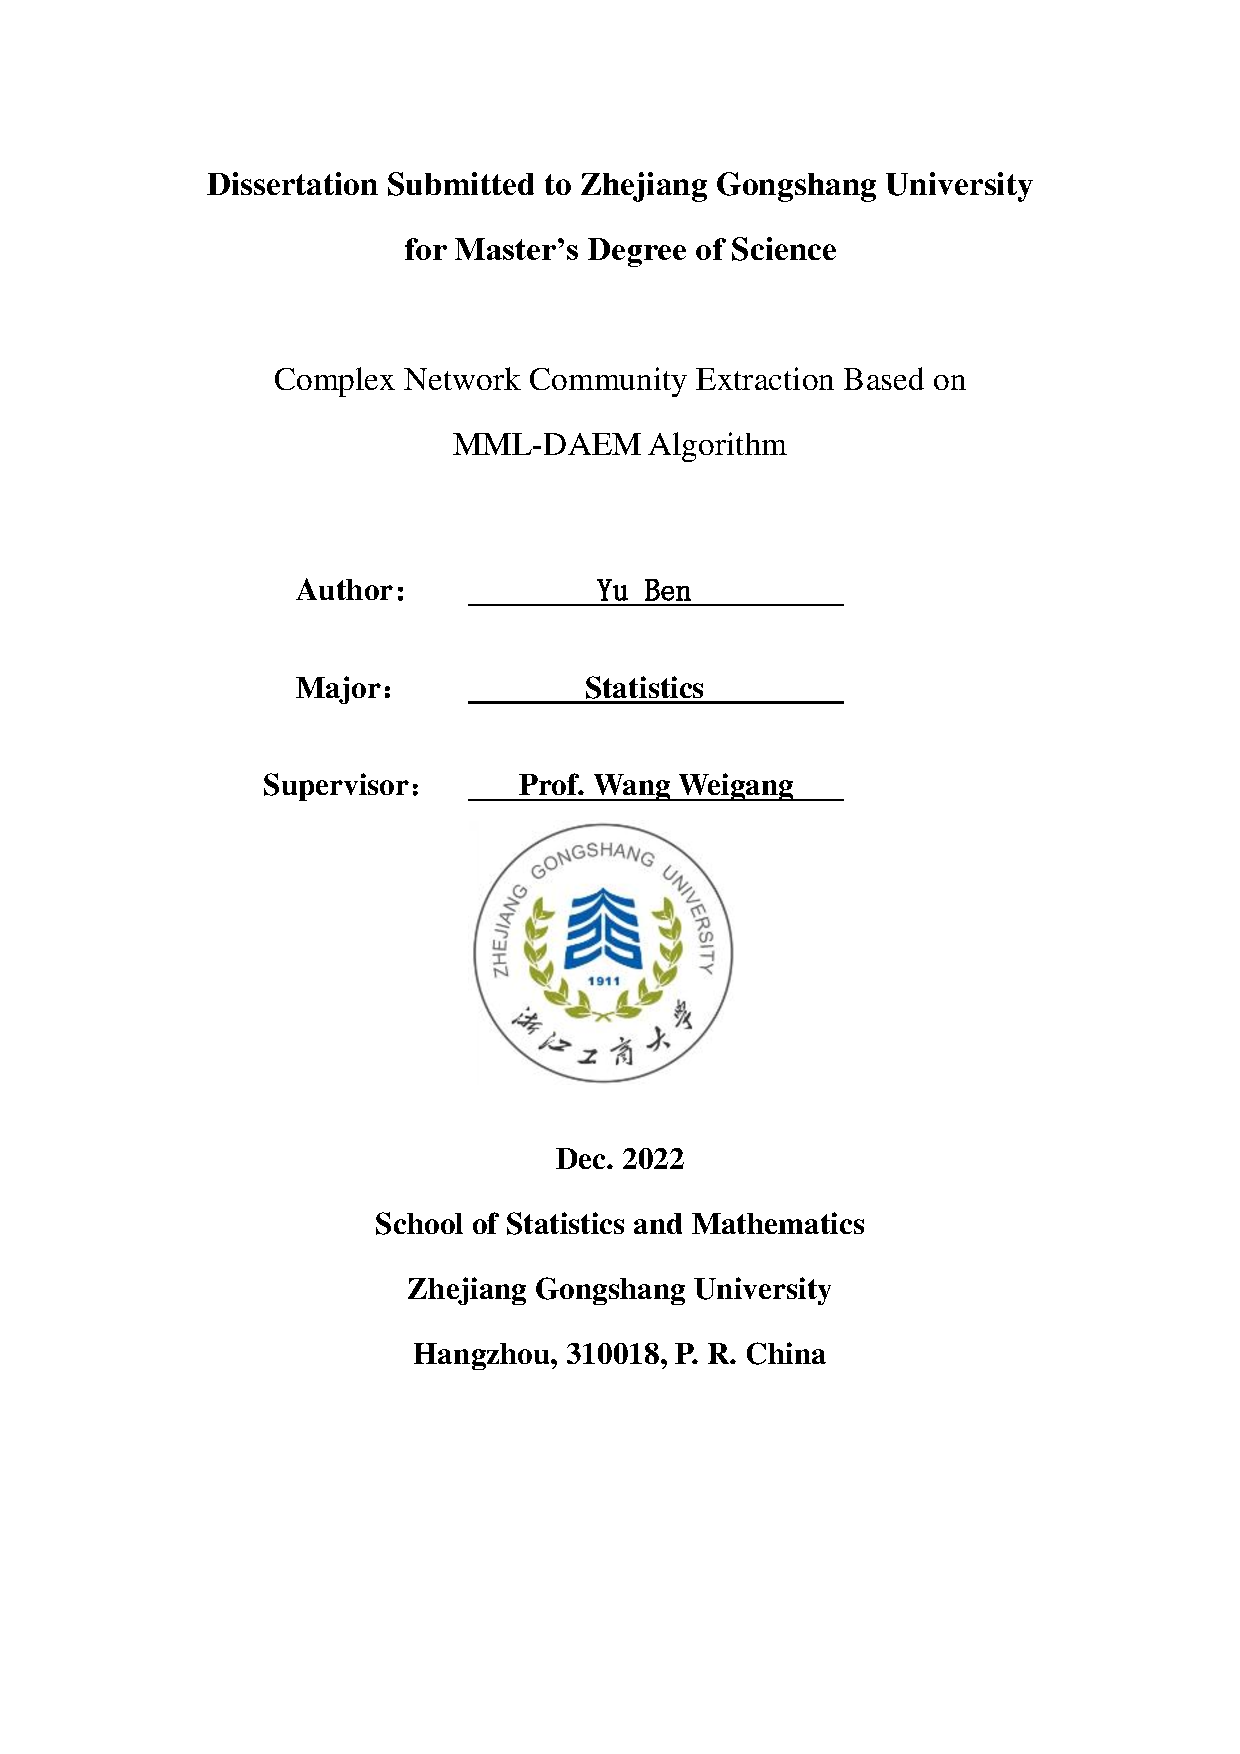
\includepdf{yingwen.pdf}
	\end{titlepage}
	
	
	%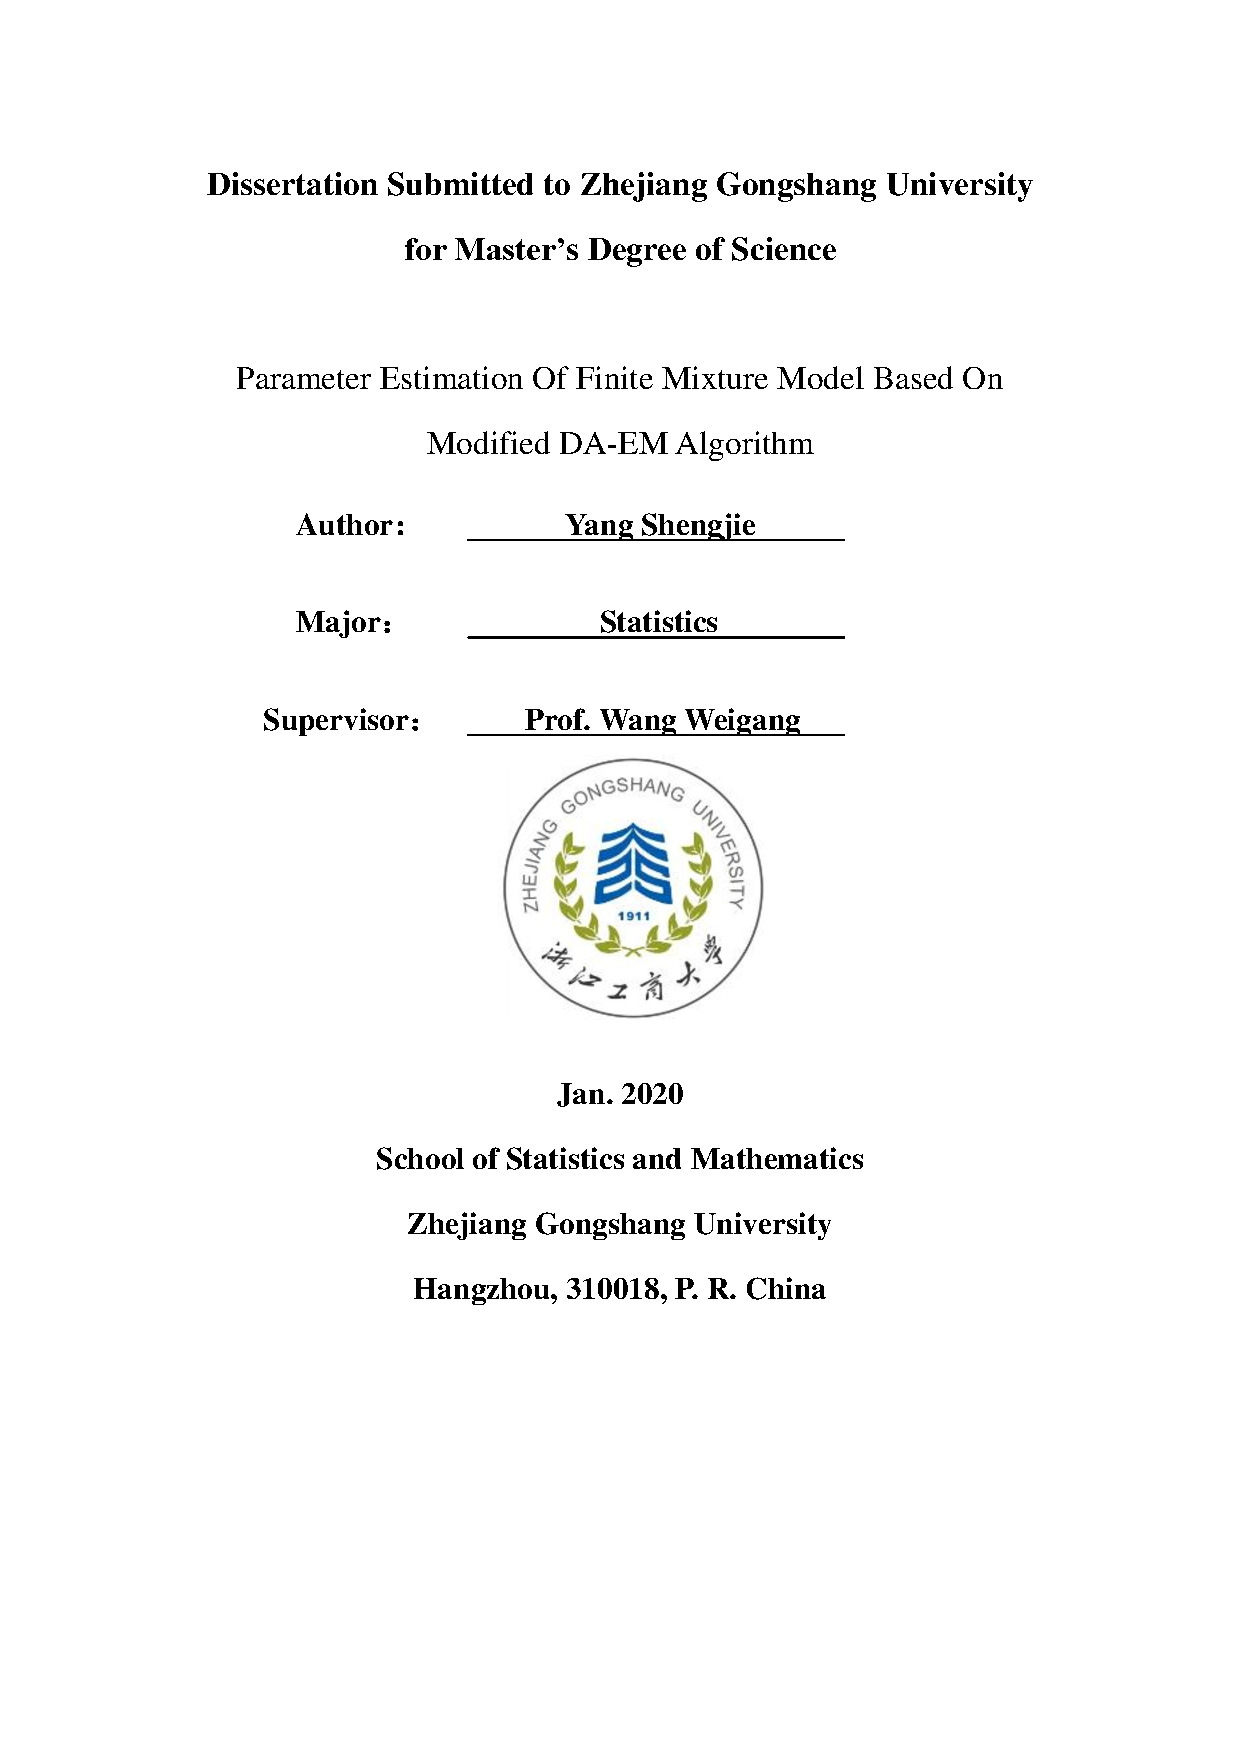
\includepdf{cover1.pdf}
	
	
	
	
	
	
	
	
	
	\frontmatter
	\pagenumbering{Roman}
	\cfoot{\thepage}
	\newpage
	\begin{center}
		\heiti\sanhao\textbf{摘\quad 要}
	\end{center}
	\hspace*{\fill} \\ %空一行
	\hspace*{\fill} \\ %空一行
	\begin{spacing}{1.5}
		{\xiaosihao\songti 复杂网络作为复杂系统最活跃的研究学科之一,由于其简明的交互系统拓扑结构的表达方式,已经被广泛应用在物理、生物和社会科学等领域。通常来说复杂网络都存在一定的社区结构,社区结构是对网络中节点的分组,组内连接相对紧密,组件连接相对稀疏。研究复杂网络的社团结构不仅有助于学者们分析复杂网络的各种潜在特性,而且与我们的生活也息息相关,比如图像分割、个性化推荐、主题分析等。复杂网络的社团检测方法有很多,寻找速度更快准确率更高的方法一直是学者们的研究内容。}
	\end{spacing}
	\begin{spacing}{1.5}
		{\xiaosihao\songti 在对各种社团检测方法进行充分研究的基础上,本文提出一种基于概率推断的MML-DAEM(Minimum Message Length-Deterministic Annealing EM)方法用于高斯混合模型的参数估计以及复杂网络的社团提取。数值模拟和实证分析结果表明本文所提出的新方法在参数估计准确度和复杂网络社团提取精度都具有优秀的结果,也为复杂网络的社团分析提供了一个新思路。}
	\end{spacing}
	\hspace*{\fill} \\ %空一行
	\noindent {\xiaosihao\songti \textbf{关键词:}高斯混合模型;DAEM算法;谱聚类;MML准则;社团提取}
	
	
	\newpage                                                            %
	\begin{center}
		\heiti\sanhao\textbf{Abstract}
	\end{center}
	\hspace*{\fill} \\ %空一行
	\hspace*{\fill} \\ %空一行
	\begin{spacing}{1.5}
		{\xiaosihao As one of the most active research subjects of complex systems, complex networks have been widely used in physics, biology and social sciences due to their concise expression of the topology of interactive systems Generally speaking, complex networks have a certain community structure. The community structure is the grouping of nodes in the network. The connections within the group are relatively tight, and the connections between components are relatively sparse Studying the community structure of complex networks not only helps scholars to analyze various potential characteristics of complex networks, but also is closely related to our lives, such as image segmentation, personalized recommendation, topic analysis, etc There are many community detection methods for complex networks, and it has been the research object of scholars to find faster and more accurate methods.}
	\end{spacing}
	
	\begin{spacing}{1.5}
		{\xiaosihao On the basis of fully studying various community detection methods, this paper proposes a MML-DAEM method based on probability inference for parameter estimation of Gaussian mixture model and community extraction of complex networks.The results of numerical simulation and empirical analysis show that the new method proposed in this paper has excellent results in parameter estimation accuracy and community extraction accuracy of complex networks, and also provides a new idea for community analysis of complex networks.}
	\end{spacing}
	
	\hspace*{\fill} \\ %空一行
	\hspace*{\fill} \\ %空一行
	\noindent{\xiaosihao \textbf{Keywords:} Gaussian mixture model; DAEM algorithm; Spectral cluster; MML criteria; Community extraction}                                                                                %
	
	%%%%%%%%%%%%%%%%%%%%%%%%%%%%%%%%%%%%%%%%%%%%%%%%%%%%%%%%%%%%%%%%%%%%%%%%%%%%%%%%%%%%%%%%%%%%%%%%%%%%%%%%
	%
	%%%%%%%%%%%%%%%%%%%%%%%%%%%%%%%%%%%%%%%%%%%%%%%%%%%%%%%%%%%%%%%%%%%%%%%%%%%%%%%%%%%%%%%%%%%%%%%%%%%%%%%%
	
	\newpage
	% 目录
	\begin{spacing}{1.8}
		\tableofcontents
		\titlecontents{chapter}[0pt]{\addvspace{2pt}\filright}
		{\contentspush{\thecontentslabel\ }}
		{}{\titlerule*[8pt]{.}\contentspage}
	\end{spacing}
	
	% 页脚
	\mainmatter
	\fancyfoot[EC,OC]{\hspace*{1 em}\thepage{}\hspace*{1 em}}
	\normalsize
	\fancypagestyle{plain}{\pagestyle{fancy}}
	\chapter[引言]{引言}\fancyhead[C]{\xiaowuhao}
	\section{研究背景及现状}
	\subsection{选题背景及意义}
	复杂系统由大量异质元素构成,并且这种元素通过各种相互作用相连。复杂网络则是对复杂系统的一种抽象。在我们的日常生活中,许多复杂系统\cite{ref1}都以网络的形式出现,不同领域更是有不同的网络,比如生态系统中的基因网络、新陈代谢网络、食物链网络,社会系统中的朋友网、姻亲关系网、Email网,信息系统中的电话线路网络、电力网、因特网等。这些网络都具有的一个特点是都具有很高的复杂性,因此这些网络统称为复杂网络。总的来说,复杂网络是研究复杂系统的一个角度和方法,它关注到系统中相互关联的作用和结构,是理解复杂系统功能和性质的一种方法。复杂网络已经成为当前各种学科交叉研究的热门领域。
	
	复杂网络的研究最早可以追溯到1736年瑞士数学家欧拉解决戈尼斯堡七桥问题。欧拉所提出的数学图论,将图抽象为顶点与边的集合,图论也成了网络研究的基础;1950年Erdos,Renyi提出的随机图论奠定了网络研究的工作基础;特别是1998年Strogatz\cite{ref2}和1999年Barabasi\cite{ref3}提出的小世界网络(Small World Network)和无标度网络(Scale-free Network)开启了复杂网络研究的热潮。
	
	复杂网络的兴起离不开计算机科学技术的发展。计算机技术的发展使我们拥有各种网络的数据库,并为大规模网络的实证研究提供了可能。其次,一些已有理论能描述和解释的普适性性质的发现也推动了复杂网络的发展,对应普适性发现的理论研究的发展的统计物理学知识、小世界网络、无标度网络都进一步推动了复杂网络的进程。
	
	除了以上特征之外,复杂网络一般还具有某种拓扑结构特性,也就是社团结构特性,表现为社团内部节点之间的联系较为稠密,社团之间的连接较为稀疏。复杂网络的社团提取就是利用复杂网络的拓扑结构,发现复杂网络所隐藏的规律,从而理解复杂网络的功能。这种研究不仅具有重要的理论意义,而且具有广泛的应用场景,比如在人际关系网中,社团结构可能是按照人的职业、年龄等组成;在引文网中不同社团代表不同研究领域;在食物链网中,社团可能反映了生态系统中的子系统等等。社团结构是中观尺度网络性质的体现,对网络中社团结构的研究是了解整个网络结构和功能的重要途径。
	\subsection{国内外研究现状}
	1970由年Kernighan B W和Lin S提出的K-L算法\cite{ref4}被认为是最早的复杂网络社团提取方法。经过不同领域各个学者几十年的研究和拓展,复杂网络社团提取的方法已经取得了相当
    快速的发展。目前为止,在社团提取方面最重要最为关键的两个问题依然是如何降低算法的时间复杂度和提升算法的准确度。更确切的说,如何在保证算法准确度的同时降低算法所需时间依然是众多学者的研究目标。早期基于非重叠的社团网络提取方法有很多,包括基于网络拓扑结构的方法,比如Grivan\cite{ref5}和Newman\cite{ref6}的GN算法、谱分析算法等。
    
    近年来,不同领域的不同学者根据应用实际需要,在原本算法基础上提出了应用于各种场景的复杂网络社团提取方法,比如基于网络动力学的Potts模型、随机游走等\cite{ref7,ref8,ref9}。从2004年至今,随着新的应用场景的出现,新的社团提取方法同样层出不穷,包括更被人所熟知的基于Q函数的优化算法\cite{ref10,ref11,ref12},其中又包括极值优化算法、快速算法、模拟退火等。
    
	还有一种是基于统计推断的方法。这类算法不仅可以识别出网络中的社团结构,还可以识别出网络结构对等的特征和规律。理论和实践均证明此类基于统计推断的方法在重组理论基础的支撑下,算法在具有较高的识别准确度的同时具有较低的运算时间复杂度。比如Newman\cite{ref13}的基于混合模型的复杂网络的探索性分析一文,将复杂网络和混合模型相结合,并且在有向和无向网络上都得到了优秀的聚类结果。其他的基于统计推断的方法包括:混合成员随机块模型(Mixed Membership Mode)和随机块模型(Stochastic Block Mode)等。这些基于统计推断的社团提取方法其实都具有相当长的计算机科学和社会科学研究史,是一种较为经典的基于生成模型的社团提取方法。
	
	国内学者对外国复杂网络的研究介绍最早可以追溯到汪小帆\cite{ref14}发表的一篇中文期刊,文中详细介绍了近几年国外在复杂网络方面所取得的进展,并介绍了相关复杂网络的概念,包括度、聚集系数、度的分布等概念,还介绍了现实世界中的英特网、科学网、小世界网络及随机网络、无标识网络等复杂网络模型。国内期刊对复杂网络的研究最早可以追溯到朱涵\cite{ref15}的“网络建筑学”一文,文中详细介绍了复杂网络的研究进程,主要包括集团化、无标识、小世界等方面。吴金闪\cite{ref16}的从统计物理学看复杂网络研究一文,从统计物理的角度分析总结出了复杂网络的研究成果,并对无向、有向、加权网络的统计性质做了归纳整理,并对小世界网络、随机网络、规则网络等网络机制做出总结。刘涛\cite{ref17}等学者从复杂网络度的分布、聚集系数等方面出发,利用其统计性质简述了小世界网络等模型的研究内容。史定华\cite{ref18}等从复杂网络度的分布切入,总结除了复杂网络模型的分类机制以及演化过程。总的来说这些研究对国内复杂网络的进一步发展壮大打下了基础。
	
	其实在实际应用中,各种社团提取方法除了前文提到的需要兼顾准确率和运行时间外,还有一个不得不考虑的问题:需要得到整个网络的拓扑结构。在网络结构较小时很容易实现,但是在构建大型网络或者动态网络的拓扑结构时,以现在的方法就很难实现。并且由于大型网络来说其复杂的拓扑结构对于计算机的良好运行也是一个挑战。因此在实际应用中,我们可以想到的方法就是利用某些具有重要信息的局部网络结构代替整个复杂网络,用局部代替总体。同样可以解决此问题的一种方法便是使用近似矩阵代替输入的向量矩阵。因此如何选取所需要的近似矩阵变成了一个新的需要解决的问题,常见的解决方法便是使用马尔科夫链蒙特卡洛(Markov Monte Carlo,MCMC)模拟。因此当前部分学者研究的热点问题便是寻找网络中某些重要节点所属的社团结构。

	\section{本文的创新点}
    1.	不同于传统的使用邻接矩阵进行聚类的方法,本文根据谱聚类提出了一种邻接矩阵的近似表示方法:利用高斯核函数RBF(Radial Basis Function)来建立邻接矩阵的近似矩阵。这种表示方法相交于传统的直接利用邻接矩阵$A$对网络结构划分的方法具有更高的准确度。
    
    2.	在对GMM(Gaussian Mixture Model)进行优化迭代时所使用的方法为EM(Expectation-Maximization)算法,由于EM算法本身的局限性,比如受初始迭代值影响、收敛到局部最优等缺点,本文在DAEM(Deterministic Annealing EM)算法的基础上,创新性的提出了基于MML(Minimun Message Length)准则的DAEM算法,解决局部最优问题和模型定阶问题。并使用所提出的MML-DAEM方法用于复杂网络的社团提取。这是由于其他人使用混合模型进行复杂网络的迭代求解时,用的迭代方法通常都是蚁群算法、遗传算法等。
    


	\section{本文组织框架}
	本文主要内容分为5章, 文章组织框架如下:
	
	第1章引言, 主要介绍了复杂网络的研究背景, 社团提取的研究现状, 并简要阐述了各种经典方法的优缺点和本文的创新点。
	
	第2章理论准备, 主要介绍了复杂网络以及社团结构的相关概念,包括复杂网络的表示、网络拓扑等相关定义,以及社团结构的各种定义和求解方法,包括基于统计模型的方法。最后介绍了如何利用谱聚类获得相似矩阵。
	
	第3章介绍的是基于高斯混合模型的社团提取方法。首先介绍了高斯混合模型及其应用场景,接着是EM算法求解GMM的求解思路与一般步骤。然后是DAEM算法包括最大熵原理,算法一般流程等。最后介绍了模型的定阶问题, 也就是确定模型的最优成分(components)数 ,主要通过MML准则进行约束。
	
	第4章模拟实证,使用现实生活中的复杂网络来验证本文所提出的复杂网络社团提取方法的准确性。
	
	第5章是总结与展望, 总结概括本文所研究的主要问题、方法及成果, 并对未来的研究工作进行安排。
	
	\begin{figure}[H]
	\centering
	% Requires \usepackage{graphicx}
	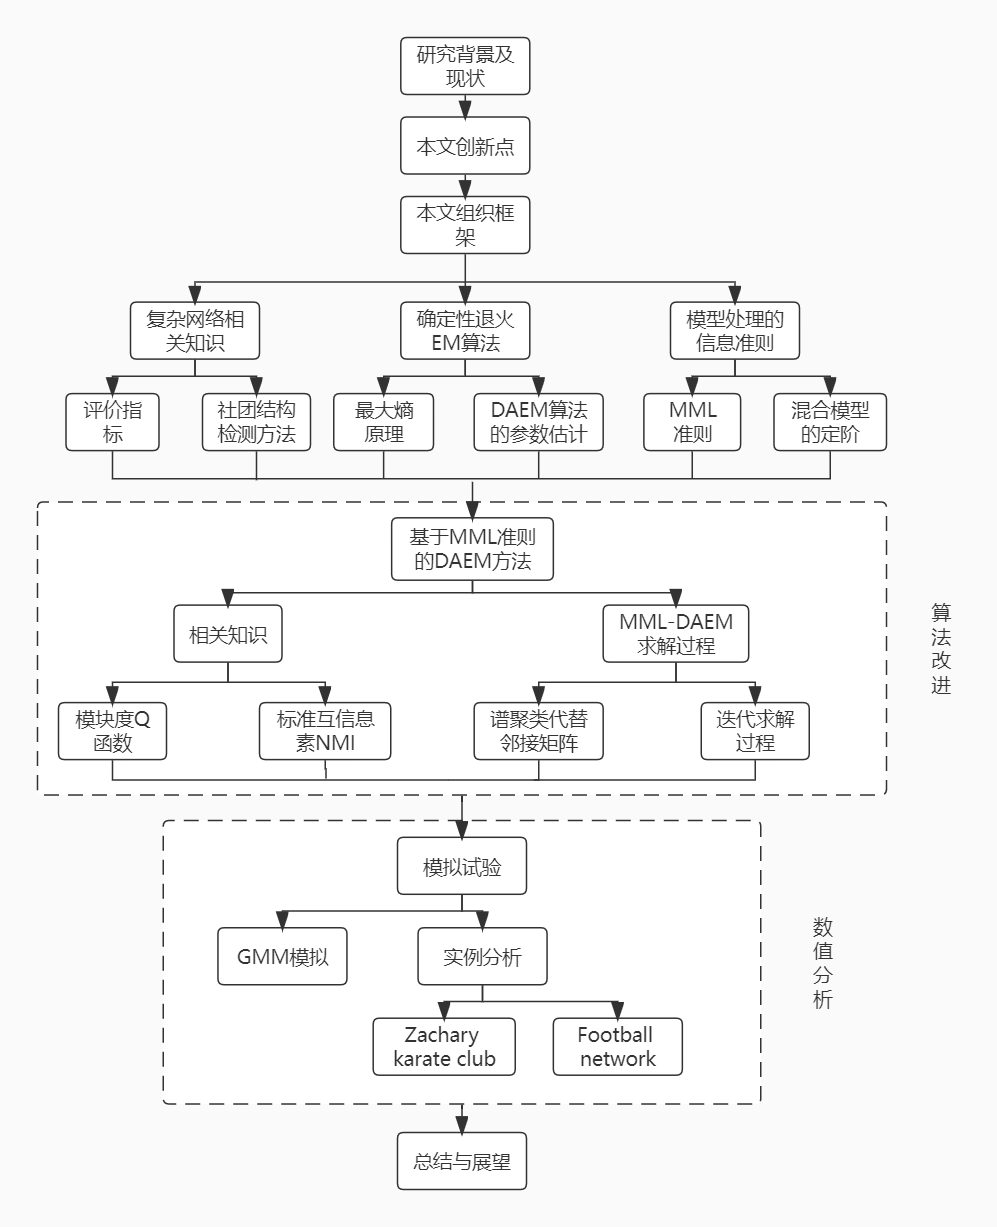
\includegraphics[width=150mm,height=180mm]{figure/流程图.jpg}\\
	\caption{论文框架流程图}\label{10}
    \end{figure}
	
	\chapter[理论准备]{理论准备}\fancyhead[C]{\xiaowuhao}
	\section{复杂网络相关概念}
	\subsection{复杂网络的表示}
    复杂网络不仅是由点及其关系组成的图,而且是关于图的集合。因此我们给出了复杂网络的图表达方式。我们知道,图包括两部分,节点和其对应关系,节点之间的相互作用我们称之为边。用数学集合的语言表示就是$G=(V,E)$,$G$表示网络,$V$表示节点集,$E$表示边集。在这样的表示方式下,网络可以分为有向,无向和加权网络。具体表示方式为:
	
    若边$e_{i}$属于$E(G)$,$(u,v)$为$V(G)$中的点集,与$e_{i}$相对于;如果任意$(u,v)$与$(v,u)$对应同一条边$e_{i}$,则称为无向网络,反之为有向网络;若任意$|e_{i}|=1$,则称为无权网络,否则称为加权网络。比如电力网就是一种有向网络,因为电力只会从发电站单向传输到用户家中,而因特网则是一种无向网络,因为用户可以通过电缆进行双向交流。
    
    复杂网络还有一种邻接矩阵的表示方法。在邻接矩阵中,对角线元素所对应的数值为0,而若两个节点之间右边存在所对应的位置取值为1,若果两个节点之间无边连接它所对应的元素取值为零。数学表达为:$A$为邻接矩阵,$A_{ij}$为邻接矩阵中的元素。
    
    在邻接矩阵的基础上,我们还可与构造邻接矩阵的拉普拉斯矩阵$L=K-A$。其中$A$为网络的邻接矩阵,$K$为一对角矩阵,对角线上的元素对应网络中各个节点的度。在实际应用中,对拉普拉斯矩阵进行特征值和特征普的分析会对我们提供很多帮助。
	\subsection{网络拓扑}
	我们知道网络是一个由多个节点组成的集合,节点之间有一定的连接方式。网络拓扑其实就是指网络节点之间相互联系的模式。比如在互联网中,节点指的是路由器,而路由器之间的连接则是通过光纤完成;比如社交网络中,节点指的是网络中的每一个单独个体人,他们之间则是通过人际关系相联系。
	\subsection{复杂网络的度}
	\textbf{复杂网络的度、平均度、度的分布}
	
	节点的度指的是与节点直接相连的边的个数。
	在邻接矩阵中,可以使用下面的方式对度进行计算:
	
	$A_{ii}=0$,$A_{ij}=A_{ji}$,那么$k_{i}$=$\sum_{j=1}^{n}A_{ij}$
	其中$A_{ij}$为邻接矩阵,$k_{i}$表示第$i$个节点的度。
	
	通常节点的度是一个离散型随机变量,我们在使用时可以计算其均值、方差等统计量:
	
	\begin{equation}
	\overline{x}=\frac{x_{1}+x_{2}+\cdots +x_{n}}{n}=\frac{1}{n}\sum_{i=1}^{n}x_{i},
	\sigma^{2}=\frac{1}{n}\sum_{i=1}^{n}{(x_i - \overline{x})^2}
	\end{equation}
	
	我们已经知道如何计算一个节点的度,那么到了某个网络的宏观方面来理解网络的性质,就需要计算这个网络的平均度$\left \langle k\right \rangle$:
	
	\begin{equation}
	\left \langle k\right \rangle=\frac{1}{n}\sum_{i=1}^{n}k_{i}=\frac{2l}{n}
	\end{equation}
	其中$l$为图中连边数,$l=\frac{1}{2}\sum_{i=1}^{n}k_{i}=\frac{1}{2}\sum_{ij}A_{ij}$
	
	通常来说具有相同度或者平均度的网络会有一些相似的性质,但是在大部分情况下它们具有不同的性质因此我们还要接着引入度分布的概念来分析网络的性质:
	
    我们将网络中节点的度值从小到大排列,统计度值为$k$的节点占整个网络节点数的比例$p(k)$,即
    
    \begin{center}
       $p(k)=\frac{n_{k}}{n}$ 
    \end{center}
    其中$n_{k}$为节点度为$k$的节点个数,$n$为节点总数。
    
    \textbf{路径、距离与介数}
    
    路径:一条路径是指一个节点序列,其中每一对相邻的节点之间都有一条连边。
    
    一条从节点$i_{0}$到$i_{n}$的长度为$n$的路径$p$经过$n+1$个节点和$n$条边。连接这两个节点的边数最少的路径叫做两个节点之间的最短路径。
    
    我们已经知道,如果节点$i$与$j$之间存在一条连边,$A_{ij}=1$,反之$A_{ij}=0$。此时$N_{ij}=1$。
    在节点$i$与$j$之间长度为2的路径数量:$N_{ij}^2$=$\sum A_{ik}A_{kj}$=$A^2_{ij}$。
    在此基础上我们可以拓展到在节点$i$与$j$之间长度为$n$的路径数量:$N_{ij}^n$=$A^n_{ij}$。
    
    \textbf{网络的介数}
    
    
    介数反映了相应的节点或边在整个网络中的作用和影响力,是一个全局几何量。介数指的是任意一对节点间最短路径所经过的次数。那么这个路径所经过的节点的次数称为点介数;如果计算的是整个路径经过某条边的次数那么所得到的就是这条边的边介数。比如在交通网中,我们通常会观察到这样一个现象,即在介数值比较高的节点可能就是交通枢纽点。

    \subsection{复杂网络的社团结构}
    社团结构一般具有三种类型:一个节点属于某一个社团的非重叠社团;一个节点可能属于多个社团的重叠社团;仅给出某些节点的社团属性的非完全分类。

    Newman\cite{ref19}首先给出了社团结构的描述性定义:社团结构(非重叠)是对网络中节点的分组,组内连接相对紧密,组间连接相对稀疏。这个定义需要满足社团连通性、具有局部相对稠密的连接密度的基本假设。
    社团结构的相关数学描述:
    
    1.	派系(Clique)
    派系指的是三个或三个以上的节点组成的全连接子图。
    
    2.k-core子图(k-core-subgraph)
    子图中的每个节点与子图内的其它节点至少有k条边相连。
    在k-core子图的基础上可以演变出k-派系社团。
    
    2.	LS集(LS-set)
    一个LS集是一个由节点构成的集合,它的任何真子集与该集合内部的连边都比与该集合外部的连边多。
    
    \textbf{社团结构的比较性定义}
    
    在比较性定义中,强社团定义为:子图$V$中任何一个顶点与$V$内部定点连接的度大于其与$V$外部顶点连接的度。即$K^i_{in}(v)>K^i_{out}(v),$$\forall i\in v$。

    弱社团的定义为:子图V中所有顶点与V内部顶点的度之和大于V中所有顶点与V外部顶点连接的度之和:
    
    \begin{equation}
        \sum_{i\in v}K^{in}_{i}(v)>\sum_{i\in v}K_{i}^{out}(v)
    \end{equation}
	
	\textbf{社团结构检测方法}:
    
    \textbf{GN算法}
    
	GN算法是Girvan和Newman提出的一种探索网络社团结构的经典分裂算法。由社团的描述性定义可知,社团指的是内部顶点连接稠密,而与其他社团的顶点连接稀疏。这就意味着社团与社团之间存在联系的通道比较少,并且想要从一个社团到令一个社团至少需要通过这些通道中的一条。那么如果可以找到这些重要的通道并把它们去除,那么网络自然会分成各个社团。以上就是GN算法的基本思想。GN算法的实现依赖着最短路径边介数,即通过每队顶点间的最短路径计算每条边被多少条最短路径通过所对应的值。
    
    \textbf{Q函数及优化算法}
    
	在GN算法中,我们会遇到一个问题,在得到分类数目不同的分类结果中,我们很难直接得到哪一个分类结果是最优的,这就需要Q函数\cite{ref20}来解决。同样由Girvan和Newman定义了模块化Q函数来衡量社团结构划分的优劣,通过Q函数来定量描述社团结构划分的模块化水平。
    
    假设网络已经被划分出社团结构,$c^i$表示顶点$i$所属的社团,则网络中社团内部连边所占的比例可以表示为:
    
    \begin{equation}
        \frac{\sum_{ij}A_{ij}\delta (c_{i},c_j)}{\sum_{ij}a_{ij}}=\frac{1}{2l}\sum_{ij}A_{ij}\delta(c_i,c_j)
    \end{equation}
    其中$A_{ij}$为邻接矩阵中的元素,$l=\sum_{ij}A_{ij}$为网络中连边的数量,$c_i$表示顶点i所属社团,当$c_i$,$c_j$属于同一个社团时,$\delta(c_i,c_j)$值为1,其它情况为0。
    
    对于社团结构固定,每个顶点的度值固定,边随机连接的网络i,j之间存在连边数的期望为:
    \begin{equation}
        \frac{k_i k_j}{2l}
    \end{equation}
    Q函数可以表示为:
    \begin{equation}
        Q=\frac{1}{2l}\sum_{i\neq j}[A_{i j}-\frac{k_i k_j}{2l}]\delta(c_i,c_j)
    \end{equation}
    其含义是网络中连接社团内部顶点之间的边的比例与拥有相同社团结构,但是顶点间随机连接的网络中连接社团内部顶点间边的比例的期望值的差值。
    如果与随机连接得到的网络没有差别,则说明这种社团结构并不显著;Q值较大时说明网络的社团结构划分是显著的。
    
    Q函数的一种等价表达方式:
    \begin{equation}
        Q=\sum_{c=1}^{n_c}[\frac{l_c}{l}-(\frac{k_c}{2l})^2]
    \end{equation}
    其中$n_c$是社团的数量,$l_c$是社团c内部所包含的边数,$k_c$是社团c中所有节点的度值之和。
    
    其推导过程如下:
    
    \begin{equation}
        Q=\frac{1}{2l}\sum_{i\neq j}[A_{i j}-\frac{k_i k_j}{2l}]\delta(c_i,c_j)
    \end{equation}
    \begin{equation}
        \frac{1}{2l}\sum_{i j}A_{i j}\delta(C_i,C_j)=\sum_{c=1}^{n_c}\frac{1}{2l}\sum_{i,j\in C_c}A_{i j}
        =\sum_{c=1}^{n_c}\frac{l_c}{l}
    \end{equation}
    \begin{equation}
        \frac{1}{2l}\sum_{i j}\frac{k_i k_j}{2l}\delta(c_i,c_j)=\sum_{c=1}^{n_c}\frac{1}{(2l)^2}\sum_{i,j\in C_c}k_i k_j=\sum_{c=1}^{n_c}(\frac{k_c}{2l})^2
    \end{equation}
    
    Q函数可以反映网络社团划分的优劣,那么便可以最大化Q函数值为目标探索网络中的社区结构,由此产生的一类新的算法:优化算法。
    常见的优化算法有贪婪算法\cite{ref21}、极值优化算法\cite{ref22}。
    
    \textbf{基于统计模型的方法}
    
    还有一种社团网络提取方法是基于统计推断的方法。基本思想是通过生成模型来模拟已知网络,将社团提取问题转化为贝叶斯推断问题,从而利用已知网络的模型假设探索模型潜在社区结构。社团提取的模型一般分为三个部分:观测变量、缺失变量(隐变量);变量的联合分布;参数$\theta$通过更新模型的参数得到观测网络的最佳拟合。
    
    最具代表性的是Newman\cite{ref16}发表的一篇文献。接下来是基于统计模型方法中的相关参数以及解释。其中$n$表示定向网络中的节点数,$A$为邻接矩阵,$A_{ij}$为邻接矩阵矩阵中的元素;$g_i$表示第$i$个节点属于哪个社团,也可以称之为隐变量,我们的目标就是推断它们来自哪个社团结构;$\theta_{r i}$表示社团r中的特定节点与节点i有连接的概率;$\pi_r$表示一个节点属于r社团的概率;$q_{i r}$表示节点i属于r社团的概率。其中$\pi$和$\theta$满足归一化条件。问题的求解需要最大化似然函数:
    \begin{equation}
          P(A,g|\pi,\theta )=P(A|g,\pi,\theta)P(g|\pi,\theta)
    \end{equation}
    其中
    \begin{equation}
        P(A|g,\pi,\theta)=\prod_{i j}\theta_{gi,j}^{A_{i j}},P(g|\pi,\theta)=\prod_{i}\pi_{g_i}
    \end{equation}
    
    由于$g$是未知的,关于参数的更新还需要用到EM算法。最后根据参数的估计结果进行迭代,输出结果是每个节点属于各个社团的概率值。
    
    \subsection{谱聚类概述}
    
    谱聚类\cite{ref23}作为一种广泛使用的聚类算法和复杂网络一样同样源自于图论,更确切的说是加权无向图。因此使用谱聚类思想研究复杂网络的社团提取是完全可行的。在上一节中,本文介绍了复杂网络的邻接矩阵$A$,在谱聚类中同样存在一个邻接矩阵$W$,不过这个邻接矩阵并不能直接得到。其基本思想是距离较远的两个数据点之间具有较低的边权重,而距离较远的点之间边权重值较高,因此需要我们在定性的原则下获得定量的权重值。解决此问题的主要方法有通过样本点度量距离的相似矩阵$S$来获得W的近似矩阵。
    
    其构建方法主要有三种:$\varepsilon $-近邻法,k-近邻法,全连接法。
    
    对于$\varepsilon $-近邻法,它设置了一个距离阈值$\epsilon$ ,接着使用欧氏距离$S_{ij}$度量两点$x_i$与$x_j$之间的距离。相似矩阵$s_{ij}=\left \| x_i-x_j\right \|_2^2$
    ,然后根据$s_{ij}$与$\epsilon$的大小关系来定义邻接矩阵$W$:
    \begin{equation}
            W_{i j}=\left\{\begin{matrix}
    0 & s_{ij}>\epsilon \\ 
    \epsilon&s_{ij}\leq \epsilon
    \end{matrix}\right.
    \end{equation}
    
    $k$近邻方法是利用KNN遍历每个样本点,然后取距离样本最近的$k$个点作为邻点,只有样本和邻点之间的$W_{i j}>0$。
    第一种$k-$近邻法只需要有一个点在另一个点的k近邻中就保留$S_{i j}$。
    \begin{equation}
        W_{i j}=W_{j i}=\left\{\begin{matrix}
    0 & x_i\notin KNN(x_j)\  and \ x_j \notin KNN(x_i)\\ 
     exp(-\frac{\left \| xi-xj\right \|^2_2}{2\sigma^2})& x_i \in KNN(x_j)\ or\ x_j\in KNN(x_i) 
    \end{matrix}\right.
    \end{equation}
    第二种$k-$近邻法需要两个点互在k近邻中保留$S_{i j}$。
    
    全连接法所有点之间的权重值都大于零,通常使用不同的核函数来定义边权重。常见的有Sigmoid核函数,多项式核函数和高斯核函数。其中最为常用的是高斯核函数RBF:
    \begin{equation}
        W_{i j}\approx S_{i j}=exp(-\frac{\left \| x_i-x_j\right \|^2_2}{2\sigma^2})
    \end{equation}
    本文在综合考量模型的复杂程度和算法难度最终选取的是高斯核函数来建立邻接矩阵的相似矩阵。
    \section{小结}
    本章主要介绍了各种理论准备。首先介绍了复杂网络的表示方法,其中基于图的表示方法是最常用的;接着介绍了复杂网络的网络拓扑结构相关定义,然后是复杂网络社团检测方法的GN算法以及Q函数优化算法;最后则是谱聚类的相关说明。
    
    \chapter{基于高斯混合模型的社团提取方法}
	\section{高斯混合模型与EM算法}
	\subsection{高斯混合模型}

    本文所研究的复杂网络社团提取问题可以理解为一个聚类问题,而聚类其目标是将样本集划分为多个类,属于无监督学习问题,目的是保证同一类的样本之间尽量相似,不同类的样本之间尽量不同。这些类称之为簇(cluster),或称之为成分(component)。与有监督分类算法不同的是,聚类算法直接完成对样本的划分而没有训练过程。
    
    基于概率分布的聚类方法前提是每个簇的样本服从相同的概率分布,也就说是一种生成模型。使用最多的是多维高斯分布,如果服从这种分布则称为高斯混合模型。求解高斯混合模型采用的方法一般为EM算法。
    
    高斯混合模型(Gaussian mixture model,GMM)通过多个高斯分布的加权之和来描述随机变量在概率空间的分布情况,其概率密度函数定义为:
    \begin{equation}\label{1}
        P(x) = \sum_{i=1}^l W_i N_i(x,\mu,\Sigma)
    \end{equation}
	其中$x$为随机向量;$l$为正态分布的数目;$w_i$为对应正态分布的权重;$\mu$为均值向量,$\sigma$为协方差向量。所有的正态分布的权重满足归一化条件:
    \begin{center}
        $\sum_i W_i=1$
    \end{center}
    
    任意一个样本$x$的产生过程可以理解为:首先从所有的$k$个正态分布中以$w_i$的概率选择出一个,再由所选择的正态分布生成样本数据。只要高斯混合模型的成分个数足够多,那么高斯混合模型就可以逼近任何一个连续的概率分布,因此它可以看作是连续型概率分布的万能逼近器。
    
    高斯混合模型的参数为:$w_i$,$\mu$,$\Sigma$。模型训练时采用的是常见的极大似然估计,其似然函数为:
    $L(\theta)=\sum_{i=1}^{l}\ln p(x_i;\theta)$,$p(x_i,\theta)=\omega_jN(x;\mu_j,\Sigma_j)$。
    
    由于对数似然函数的复杂性,混合模型无法像单个正态模型那样求得公式解,如果使用最优化方法求解,比如牛顿法、梯度下降法,求解过程同样困难,因为$w_i$需要满足等式和不等式约束。如果换个角度来看,要是知道每个样本所属的高斯分布,问题就会变简单,需要做的就是分别估计$k$个高斯分布的参数,利用标准的极大似然估计就能完成,得到均值和协方差向量的估计值。但是同样的,每个样本属于哪个高斯分布未知,而我们在计算参数的估计值时会用到这个信息,反过来,样本属于哪个高斯分布是由高斯分布的参数决定。因此存在着依赖循环,为了解决这个问题只能打破这个循环,即需要从高斯分布的一个随机初始值开始,计算样本属于每个高斯分布的概率,然后根据这个概率更新参数。这便是EM算法的求解思路。
    
    \subsection{EM算法}
    
    EM算法\cite{ref24}即期望最大算法(Expectation Maximum algorithm),是一种迭代法,它可以估计出每个样本所属簇的类别以及每个簇的概率分布函数。如果要聚类的样本数据服从它所属的簇的概率分布,则可以通过估计每个簇的概率分布以及每个样本所属的簇来完成聚类。估计每个簇概率分布的参数需要知道哪些样本属于这个簇,从而确定每个样本属于哪个簇又需要知道每个簇的概率分布的参数,这存在着依赖循环。EM算法在每次迭代时交替地解决上面的两个问题,直至收敛到局部最优解。
    
	在介绍算法之前需要先介绍Jensen不等式。假设$f(x)$是凸函数,$x$是随机变量,那么不等式满足:
    \begin{center}
        $E (f(x))>f (E(x))$
    \end{center}
	
	若$f(x)$是一个严格凸函数,那么当且仅当$x$为常数时不等式取等:
    \begin{center}
        $E (f(x))=f (E(x))$
    \end{center}
    
	EM算法作为一种迭代法,其解决问题时求解后验概率或者似然函数的极值,而样本中具有没法直接观测的隐变量。比如,我们有一个属于三个类的一批样本,这三个类都服从均值和协方差未知的高斯分布,并且样本属于哪一类同样未知。我们需要在这种情况下估计出每个高斯分布的参数。其实,样本所属的类就可以看作是隐变量,从而导致极大似然估计在求解时遇到困难。
    
    假设我们从$p(x,\theta)$生成了包含观测数据$x_i$的$l$个样本,$z_i$为无法直接观测的隐变量,$\theta$为概率密度函数的参数,是未知的。需要做的是根据样本估计出参数$\theta$。我们可以构造似然函数利用极大似然估计进行分析:
    \begin{equation}
        L(\theta)=\sum_i \ln p(x_i,\theta)=\sum_i \ln\sum_{z_i}p(x_i,z_i;\theta)
    \end{equation}
    
    $z_i$是隐变量,同时也是一个离散型随机变量。由于隐变量的存在,我们无法直接求得似然函数极大化后参数的公式解,但是可以换种思路,我们可以构造出一个更容易优化的似然函数的下界函数,然后优化所构造的下界函数。以下界函数的值不断增加为目的不断改变优化变量的值,从而使得似然函数的值增加,这也是EM算法的思路。
    
    假设$q(z_i)$为$z_i$的概率分布,利用这个概率密度函数,我们可以将似然函数进行变形:
    
    \begin{center}
    $q(z_i)=p(z_i|x_i,\theta_t)$
    \end{center}
    由于$q_i$可以是任意个概率分布,计算时可以按照如下公式:
    
    \begin{equation}
        q_i(z_i)=\frac{p(x_i,z_i;\theta)}{\sum_{z_i}p(x_i,z_i;\theta)}
    \end{equation}
    
    现在可以总结出EM算法的一般步骤:
    
    输入:观测数据$X$,隐变量数据$Z$,联合分布$P(x,z|\theta)$,隐变量分布$P(z|x,\theta)$
    输出:参数$\theta$的估计值。
    
    E步:记$\theta^i$为第$i$次迭代$\theta$的估计值,在第$i+1$次迭代中,计算
    \begin{equation}
      Q(\theta,\theta^{i})=E_z[logP(x,z|\theta)|x,\theta^{i}] 
    \end{equation}
    
	M步:求解使得Q函数极大化的参数$\theta$,第$i+1$次迭代的估计值
    $\theta^{i+1} = \ \underset{\theta}{max} Q(\theta,\theta^{i}$
	重复步骤2,3直到收敛。
	
	由于E步目标函数没有求和项,因此更容易求得$\theta$的公式解。同时我们可以得到用EM算法求解高斯混合模型的算法流程。首先初始化$\boldsymbol{\mu,\Sigma,\omega}$,接着进行循环迭代,直到算法收敛。迭代停止的判定规则为相邻两次函数值之差小于给定阈值或者算法迭代到给定次数。每次迭代执行的操作为:
	
	E步,根据当前模型参数的估计值,计算第i个样本来自第j个高斯分布的概率:
	\begin{equation}
	    q_{ij}=p(z_i=j|\boldsymbol{x_i;\omega,\mu,\Sigma})
	\end{equation}
    
    M步,计算模型的各个参数:
    
    \begin{equation}
        \omega_j=\frac{1}{l}\sum_{i=1}^l q_{i j}
    \end{equation}
    
    \begin{equation}
        \mu_j=\frac{\sum_{i=1}^l q_{i j}x_i}{\sum_{i=1}^l q_{i j}}
    \end{equation}
    
    \begin{equation}
        \Sigma_j=\frac{\sum_{i=1}^l q_{i j}(x_i-\mu_j)(x_i-\mu_j)^T}{\sum_{i=1}^l q_{i j}}
    \end{equation}
    
    $q_{i j}$是根据参数当前的估计值计算出来的对$z_i$的概率分布的猜测。可以使用贝叶斯公式和全概率公式计算$q_{i j}$:
    
    \begin{equation}
        p(z_i=j|x_i;\omega,\mu,\Sigma)=\frac{p(x_i|z_i=j;\mu,\Sigma)p(z_i=j;\omega)}{\sum_{c=1}^k p(x_i|z_i=c;\mu,\Sigma)p(z_i=c;\omega)}
    \end{equation}
    
    迭代终止条件为达到指定迭代次数或者相邻两次迭代似然函数值小于给定阈值。下面我将给出算法收敛性的简单证明。我们假设第$t$次迭代时其参数为$\theta_t$,第$t+1$次迭代时的参数为$\theta_{t+1}$。如果能够说明$L(\theta_t)\leq L(\theta_{t+1})$,即似然函数值递增,则算法可以收敛。
    
    由于
    \begin{equation}
        q_{i j}=P(z_i|x_i,\theta_t)
    \end{equation}
    故
    \begin{equation}
        \frac{p(x_i,z_i;\theta_t)}{q_{i j}(z_i)}=\frac{p(x_i,z_i,;\theta_t)}{p(z_i|x_i;\theta_t)}=p(x_i;\theta_t)
    \end{equation}
    
    是一个与$z$无关的常数,因此Jensen不等式可以取等。下面的等式也就成立
    \begin{equation}
        L(\theta_t)=\sum_i \ln\sum_{z_i}q_{i t}(z_i)\frac{p(x_i,z_i;\theta_t)}{q_{i t}(z_i)}=\sum_i\sum_{z_i}q_{it}(z_i)\ln \frac{p(x_i,z_i;\theta_t)}{q_{i t}(z_i)}
    \end{equation}
    有
    \begin{equation}
    \begin{aligned}
        L(\theta_{t+1}) & \geq \sum_i\sum_{z_i}q_{i t}(z_i)\ln \frac{p(x_i,z_i;\theta_{t+1})}{q_{it}(z_i)} \\ 
        & \geq \sum_i\sum_{z_i}q_{i t}\ln \frac{p(x_i,z_i;\theta_t)}{q_{i t}(z_i)} \\ 
        &=L(\theta_t)
    \end{aligned}
    \end{equation}
    
    由上式计算可知每次迭代时似然函数值都会增加,一直到极值点出现为止。需要说明的是其收敛得到的极值点很可能只是局部极值点。
    
    \section{确定性退火EM算法与GMM}
    为了解决EM算法收敛到局部最优解的问题,Ueda\cite{ref25}等提出了确定性退火EM算法(Deterministic annealing EM algorithm)。在文章中,作者利用最大熵原理导出了一个新的“温度”后验参数,并用于控制退火过程。在DAEM算法中,他们将对数似然最大化的问题重新表述为由最大熵原理和统计力学类比定义的热力学自由能最小化问题,并在退火参数逐渐增加时新的算法迭代的初始值是上一次迭代得到的局部最优的参数值,并进行下一轮迭代。
    \subsection{最大熵原理}
	熵(entropy)首先由Clausius于1865年提出,泛指某些物质系统状态可能出现的程度。1948年Shannon将物理学中熵的概念引申到了通信过程中,并创立了信息论这门学科,将熵推广为信息熵。
	在信息论于概率统计中,信息熵表示随机变量不确定性的度量。假设$X$是一个离散型随机变量,其概率分布函数为:
    \begin{center}
        $P(X=x_i)=p_i,i=\cdots,n$
    \end{center}
    那么随机变量$X$的信息熵为:
    \begin{center}
    $H(x)=-\sum_i p_i log_{p_i}$
    \end{center}
    
    由定义可知,熵的大小于随机变量的取值无关,只依赖其分布,故随机变量X的熵可以表示为:
    \begin{center}
    $H(p)= -\sum_i p_i log_{p_i}$
    \end{center}
    
    熵越大则表示相应随机变量的不确定性越大。

    而最大熵原理由Jaynes\cite{ref26}提出,最大熵原理是概率统计学习中的一个准则。最大熵原理的思想是:在学习统计模型的概率分布时,在所有满足条件的概率分布中,熵最大的模型是最好的。最大熵原理通常会存在约束条件,利用约束条件来确定概率分布模型的集合,因此最大熵原理也可以理解为在约束条件下寻找熵最大的模型。随机变量$X$的信息熵满足:
    
    $0\leq{H(p)}\leq{logN}$,$N$为$X$的取值个数,并且当且仅当$X$服从均匀分布时取等,并且此时熵最大。
    
	简单来说,最大熵原理认为必须在已有的事实中选取需要的概率模型,即满足约束条件,在没有更多已知信息时,哪些未知的部分认为是等可能的,而这种“等可能”的满足需要通过熵的最大化来完成。“等可能”很难直接完成,而信息熵则是一个可以优化的数值指标。
	
    和EM算法不同的是,DAEM算法使用了一个新的后验概率$f(z|x,\theta)$来代替隐变量的分布函数$q(z_i)$。在DAEM算法中,关于$f$的形式将在后面给出。同时使用一个新的E函数代替E步的Q函数:
    \begin{equation}\label{eq1}
        E\overset{def}{=}\sum_{k=1}^{N}[-logp(x_k,y_k;\Theta)]f(y_k|x_k)dy_k。
    \end{equation}
    
    E函数通常非负,并且也是一个条件期望,如果$p=f$,那么$E=-Q$。由于我们任何关于$f$的先验知识,因此采用最大熵原理求解,通过最大化下式的熵:
    \begin{equation}\label{eq2}
        H=-\sum_k\int[log\ f(z_k|x_k)]f(z_k|x_k)dz_k
    \end{equation}
    限制条件为equationE,$\int f dz=1$,通过构造拉格朗日函数求得f的Gibbs分布:
    \begin{equation}\label{eq3}
        f(z_k|x_k)=\frac{1}{Z_x}exp[-\beta(-log\ p(x_k,y_k;\theta))]
    \end{equation}
    
    $Z_x=\int \exp[-\beta(-logp(x_k,z_k;\theta))]dz_k$为partial function,参数$\beta$是拉格朗日乘子,由E的值决定,$\frac{1}{\beta}$对应着退火理论中的温度T。通过简化上式,可以得到一个关于$\beta$的后验概率:
    \begin{equation}\label{eq4}
        f(z_k|x_k)=\frac{p(x_k,z_k;\theta)^\beta}{\int p(x_k,z_k;\theta)^\beta dz_k}
    \end{equation}
    和原始EM算法不同的确定性EM算法加入了一个参数$\beta$去模拟退火过程。但是DAEM算法和模拟退火方法不同的一个重要区别是DAEM算法对每一个$\beta$所做的优化是确定性的。模拟退火过程以一个小的$\beta$作为初始值代表着高的温度,很明显在此时$f(z_k|x_k)$一致连续,$H$只有一个全局最大值,因此最大值很容易被找到。接着当主键增加参数$\beta$时,每一个$x_k$的影响将逐渐边缘化。当$\beta>0$,函数$H$将会有多个局部最大值,在每一步中,都可以假定新的全局最大值接近于前一个步骤的局部最大值。因此通过这个假设该算法可以在$\beta$增加时追踪到每个$\beta$的全局最大值。当$\beta$等于1时,$f$和EM算法中关于隐变量$z$的后验概率$p$相同,此时DAEM算法则退变为EM算法。$\beta$的最大值不能超过1。因此可以将EM算法看成是DAEM算法的一个特例。在DAEM算法中,作者将求解最大对数似然函数问题转变为求解最小自由能函数问题。 DAEM算法在后验概率的求解上引入了退火参数$\beta$:\begin{equation}\label{eq5}
		\varphi_{i k}=\frac{\omega_j N(x_i;\mu_j,\Sigma_j)^\beta}{(\sum_{t=1}^k\omega_t N(x_i;\mu_t,\Sigma_t))^\beta}.
	\end{equation}
	对于高斯混合模型来说, 如果$\omega_{i k}$已知, 那么~$\theta=\left(\left(\alpha_{1}, \mu_{1}, \Sigma_{1}\right), \cdots,\left(\alpha_{K}, \mu_{K}, \Sigma_{K}\right)\right)$~的最大似然估计与EM算法相同\begin{equation}\label{eq6}
		\omega_{k}=\frac{\sum_{i=1}^{n} \varphi_{i k}}{n},
	\end{equation}\begin{equation}\label{eq7}
		\mu_{k}=\frac{\sum_{i=1}^{n} \varphi_{i k} x_{i}}{\sum_{i=1}^{n} \varphi_{i k}},
	\end{equation}\begin{equation}\label{eq8}
		\Sigma_{k}=\frac{\sum_{i=1}^{n} \varphi_{i k}\left(x_{i}-\mu_{k}\right)\left(x_{i}-\mu_{k}\right)^{T}}{\sum_{i=1}^{n} \varphi_{i k}}.
	\end{equation}
	
	接着我将解释DAEM算法如何在不受初始值的影响下收敛到一个次优解的。等式3-18表明退火参数$\beta$平滑了自由能函数\cite{ref21},在$\beta$增加时平滑率也在增加。当$\beta$足够小时,自由能函数会有一个全局最小值,并且可以通过EM算法计算得到。那么在温度减少即$\beta$增加时,密度函数的效应将逐渐增强并且将会出现在自由能函数的局部极小值。因此在不同的$\beta$的每一个循环,自由能函数值都会变化,新的全局最小值将会接近上一个值,因此该算法可以找到新的全局最小值。但是,在实际应用中以上讨论并不总会成立详细讨论可以参考Ueda N和Nakano R\cite{ref21}的文章。那么在这种情况下 DAEM算法将会收敛到全局次优点。也就是说,一个新的全局最优点接近于先前跟踪的全局最优点时,DAEM算法才能保证全局最优。
	关于模型参数$\beta$的初始值选取,参考Ueda\cite{ref21},将$\beta_0$设置为0。5,$\beta_{new}=\beta_{current}\times 1.2$。关于EM和DAEM算法中高斯混合模型参数初始值主要有两个方法:随机初始化和使用K-means初始化。
	DAEM算法的流程如下:
    
    \begin{algorithm}
	\caption{基于DAEM算法的高斯混合模型参数估计方法} %算法的名字
	\hspace*{0.02in} {\bf Input:} %算法的输入,  \hspace*{0.02in}用来控制位置, 同时利用 \\ 进行换行
	观测数据$X=\left\{x_{1}, \ldots, x_{n}\right\}$, 高斯混合模型,$\epsilon_{1},\epsilon_{2}>0$, 初始退火参数$\beta\leftarrow\beta^{0}$, $t=0$\\
	\hspace*{0.02in} {\bf Output:} %算法的结果输出
	高斯混合模型参数$\theta=\left(\left(\omega_{1}, \mu_{1}, \Sigma_{1}\right), \cdots,\left(\omega_{K}, \mu_{K}, \Sigma_{K}\right)\right)$
	\begin{algorithmic}[1]
	\State 参数初始值$\theta^{(0)}=\left(\left(\omega_{1}^{(0)}, \mu_{1}^{(0)}, \Sigma_{1}^{(0)}\right), \cdots,\left(\omega_{K}^{(0)}, \mu_{K}^{(0)}, \Sigma_{K}^{(0)}\right)\right)$ % \State 后写一般语句
			
	\While{$\beta \leq 1$} % While语句, 需要和EndWhile对应
	\State 根据式\ref{eq5}计算后验概率$\varphi_{i k}$, 即每个分模型对观测数据的响应度;
	\State 根据式\ref{eq6}, \ref{eq7}, \ref{eq8}计算当前混合模型的参数;
	\State 判断两次迭代的最大似然估计参数不在变化, $\left\|\Theta^{(t+1)}-\Theta^{(t)}\right\|<\epsilon_{1}$, 或者Q函数不再变化, $\left\|Q\left(\theta^{(t+1)},\theta^{(t)}\right)-Q\left(\theta^{(t)},\theta^{(t)}\right)\right\|<\epsilon_{2}$. 否则, $t=t+1$, 重复步骤3,4;
	\EndWhile
	\end{algorithmic}
	\end{algorithm}
	
	
	
    \subsection{混合模型的定阶}
    在前几章本文主要介绍了复杂网络和EM算法及其参数估计的相关知识,但是在实际应用中的混合模型成分数往往是不确定的,它需要根据各个成分的密度参数从样本中推断。在GMM中,成分数量之所以难确定主要是因为太多的成分会使得模型过拟合,从而使得模型的泛化能力变差;而成分数太少则很难发现隐藏在数据中的规律。所以混合模型的成分选择也就是定阶问题一直是一个非常重要但又难以解决的问题。
    
    在混合模型的聚类分析中,关于成分数的确定不同学者提出了不同方法\cite{ref27},主要分为三个方面:1.图形化技术和视觉审查2.假设检验3.模型准则。通过使用足够多的成分数,总能找到一个合适的拟合,但是它是否合理则是我们需要着重考量的。图形化技术比如直方图和概率图是在多个候选值中挑选一个合适的。然而对这些图形的视觉审查表明这并不是一个合理的方法,比如一个单峰分布可能含有多个成分。由Wolfe\cite{ref28}提出的使用$\chi ^2$统计量的假设检验同样被证明不合理。在现阶段,大多推断混合模型成分个数的方法都是将确定成分数问题和模型参数估计问题相分离,即先确定成分$k$的范围,估计模型的参数,然后使用某一评价标准选择评价指标最好的成分数作为最优成分个数。这些评价标准包括:

    Minimun message length(MML)\cite{ref29}
    
    Partition coefficient(PC)\cite{ref30}
    
    Akaike's information criterion (AIC)\cite{ref31}
    
    ICOMP\cite{ref32}
    
    Minimum description length (MDL)\cite{ref33}

    最优成分数的确定往往还是要通过极大似然估计来实现。由于最大似然方法本身并不能确定最优成分数,因此这些评价标准的实现主要是通过在似然函数中加入一个惩罚项。并且似然函数通常是成分数$k$的非减函数,这就是所谓的对数似然罚函数方法。由于这些方法通常是基于信息编码概念原理的,因而也称为信息准则。这些准则对数据和模型的要求低,计算量少,因此受到很多学者喜爱。

    \subsection{模型选择的信息准则}
    
	我们已经知道选择最优成分数是通过引入一个关于成分数的惩罚形式的似然函数,通过计算尽可能多的计算不同成分$k$的似然函数的某种准则的函数值,然后找到对应函数值最小(或最大)对应的$k$值即为混合模型的成分数。并且似然函数通常为$k$的非减函数,因此需要加入惩罚项防止函数值一直变大(变小)。其最优成分准则通常为:
	\begin{equation}
	    \hat{h}=arg min\{C(\hat{\theta}(h),h),h_{min}\leq h\leq h_{max}\}
	\end{equation}
    其中$C(\theta(h))$为某种模型选择函数。其形式通常为:
    \begin{equation}
        C(\hat{\theta}(h),h)=-logL(\hat{\theta}(h))+\psi (h)
    \end{equation}
    其中$L$为似然函数,$\psi$为惩罚函数,随$h$递增。比如经常使用的基于AIC(Akaile’s information criterion)的信息准则:
    \begin{equation}
        AIC(h)=-logL(\hat{\theta}(h))+P(h)
    \end{equation}
    其中$p(h)$是模型的成分为$h$时(自由)参数的个数。
    Wallace and Freeman\cite{ref32}给出了MML(minimum message length)的一般形式:
    \begin{equation}\label{eq9}
       MMLen\approx \frac{n_p}{2}-logh(\theta)-\frac{n_p}{2} \log k_{n_p}+\frac{1}{2}\log det(F(\theta)\\-logf(x|\theta)
    \end{equation}

    其中$h(\theta)$为关于参数值的先验分布,$F(\theta)$为期望费希尔信息矩阵,$f(x|\theta)$为混合模型的对数似然函数,$n_p$为需要被估计的参数个数,$K_{n_p}$为$n_p$维的最优quantizing lattice常数,其中$k_1=\frac{1}{12}$,$k_2=\frac{5}{36\sqrt{3}}$。$K_{n_p}$的值可参考Conway and Sloane\cite{ref33}的表2.3。但其实$k_{n_p}$之间在$n_p$不是特别大时实际差别并不大,因此还可以将其统一设置为$\frac{1}{12}$,具体可以参考连军艳\cite{ref34}。
	为了得到等式\ref{eq9}的具体表达形式,我们首先需要选择一个$h(\theta)$的先验分布,然后获得$F(\theta)$即费希尔信息矩阵行列式的表达式。
	
	我们采用和Wallace和Boulton\cite{ref29}相同的关于$w_i$,$\mu_i$和$\sigma_i$的先验分布。我们对$w_i$采用了均匀先验的形式:
	
    \begin{equation}
        h(\tilde{w})=(k-1)!,\sum_{i=1}^k w_i=1,0\leq w_i\leq 1,\forall i=1\cdots k
    \end{equation}
	对于$\sigma$我们采取一个范围在0和$\sigma_p$之间的均匀先验形式:
	
	\begin{equation}
	    h(\sigma_i)=\frac{1}{\sigma_p},\    0\leq \sigma_i\leq \sigma_p, \   i=1\cdots k
	\end{equation}
	$\sigma_p$为总标准差。
	
	我们同样在总体标准差范围内采用$\mu_i$的先验分布:
	
	\begin{equation}
	    h(\mu_i)=\frac{1}{2\sigma_p}
	\end{equation}
	
	对于$\mu_p-\sigma_p\leq \mu_i \leq \mu_p+\sigma_p,i=1\cdots k$。我们假定对于$k$的取值,$k=1$到$k=K$是等可能的。因此某一个值$k$的信息长度将和其他$k$的一样,并且可以被忽略。
	
	我们假定所有的参数均是独立的,因此:
	
	\begin{equation}\label{eq10}
	    h(\theta) = \frac{(k-1)!}{2^k\sigma_p^{2k}}
	\end{equation}
	
	选取等式\ref{eq10}作为参数$\theta$先验分布理由如下:
	
	1.	此先验分布具有位置和尺度不变性。也就是说如果我们以线性的方式改变测量单位得到的同样是一个先验分布,因此结果等价。
	
    2.	本文已经解释了一个关于$p_j(\alpha)$的均匀先验。先验分布的均值和标准差表明,我们已知关于它们值的大致估计,并不知道它们的实际值。
    
    \textbf{费希尔信息矩阵行列式的估计}
    
    具有多个成分的费希尔信息矩阵很难直接得到。因此,我们将费歇尔信息矩阵的行列式近似为每个分量的费歇尔信息矩阵的行列式,乘以关于$p_j$的费歇尔信息矩阵的行列式:
    \begin{equation}\label{eq11}
        de t (F(\theta))\approx \prod_{i=1}^{k}det (F_i(\mu_i,\sigma_i))\times det (F(w))
    \end{equation}
    其中具有均值向量$\mu_j$和标准差向量$\sigma_j$的单个高斯分布的Fisher信息矩阵为:
    
    \begin{equation}\label{eq12}
        F_i(\mu_i,\sigma_i)=\begin{bmatrix}
    \frac{n_i}{\sigma_i^2} &0 \\ 
    0 & \frac{2n_i}{\sigma_i^2}
    \end{bmatrix}
    \end{equation}
    其中$n_j=W_j\times n$为成分$j$的期望items数量。因此
    \begin{equation}\label{eq13}
        det(F_i(\mu_i,\sigma_i))=\frac{2n_i^2}{\sigma_i^4}
    \end{equation}
    $p_i$可以看作是一个多项式分布的参数,因此
    \begin{equation}\label{eq14}
        det(F(p))=\frac{n}{\prod_{i=1}^{k}p_i}
    \end{equation}
    将等式\ref{eq13},\ref{eq14}带入到\ref{eq12}中,最终得到:
    \begin{equation}\label{eq15}
        \frac{1}{2}log\ \det(F(\theta))\approx \sum_{i=1}^{k}log\frac{\sqrt{2}n_i}{\sigma_i^2}+\frac{1}{2} log\ n\\ -\frac{1}{2}\sum_{i=1}^{k}log\ p_i
    \end{equation}
    由于我们描述成分参数时是以某种顺序的,并且每个成分被描述的顺序是不相关的,因此需要减去这部分的值。在标记其成分数时一共有K!个排列,其对应的信息长度为:
    \begin{center}
        $log\ k!$
    \end{center}
    综上,
    
    \begin{equation}
    \begin{aligned}
    MMLen &\approx -\frac{n_p}{2}log k_{n_p}+\frac{n_p}{2}\\&-k log\frac{1}{2\sigma_p^2}-log(k-1)!\\&+\sum_{i=1}^k log\frac{\sqrt{2}n_i}{\sigma_i^2}+\frac{1}{2}log\ n\\&-\frac{1}{2}\sum_{i=1}^klog\ p_j-log\ f(\tilde{x}|\theta)-logk!
    \end{aligned}
    \end{equation}
	本文所提到的相关信息准则(PC,AIC,MDL,ICOMP,MML)都可以推广到多维数据(假定每个样本$x_j$都是M维),如果我们假设每个分量都是一个具有对角协方差矩阵的多元高斯分布,第$j$个成分中的参数为:
	\begin{center}
	    $w_j,\ \mu_{j1},\cdots \mu_{jM}\ \sigma_{j1},\cdots \sigma_{jM} $
	\end{center}
	
	估计这些参数时同样使用EM迭代法,不过各参数也需要做一些改变:
	
	\begin{equation}
	    \mu_{im}=\frac{\sum_{j=1}^l q_{ij}x_{j m}}{\sum_{j=1}^l q_{ij}}
	    \Sigma_{i m}=\frac{\sum_{j=1}^l q_{i j}(x_{j m}-\mu_{im})(x_{jm}-\mu_{im})^T}{\sum_{j=1}^l q_{i j}}
	\end{equation}
	
	对于MML准则,我们还必须将等式\ref{eq10}的先验值替换为:
	
	\begin{center}
	   $ h(\theta)=\frac{(k-1)!}{2^{m k}}\prod_{m=1}^{M}(\frac{1}{\sigma^p})^{2k}$
	\end{center}
	
	最后还需要替换等式\ref{eq11}中的费歇尔信息矩阵的行列式:
	
	\begin{equation}
	\begin{aligned}
	    \frac{1}{2}\log det(F(\theta))&\approx\frac{1}{2}\log n-\frac{1}{2}\sum_{i=1}^k\log p_i\\&+\sum_{m=1}^M\sum_{i=1}^k \log\frac{\sqrt2n_j}{\sigma_{i m}^2}
	\end{aligned}
	\end{equation}
	
	\subsection{MML-DAEM算法}
	
	首先我将把DAEM算法和复杂网络结合起来。
	
	假设有一个$n$个节点的网络,该网络可以使用邻接矩阵$A$进行数学描述。如果有某个点属于某个社团或组,也就是GMM中的成分,我将使用$g_i$表示顶点$i$所属的组。通常$g_i$不能直接衡量得到,它对应着混合模型中的隐变量。本文的目标之一就是通过网络结构去推断出它的具体值。接着我将定义$\theta_{r i}$为组$r$中某个特定节点和节点$i$相连接的概率,节点$i$既可以在组$r$内,也可以在组外。因此,我们所设想的结构可以与传统的分类混合网络有很大的不同,尽管它是分类混合模型的一种特殊情况。接着我将定义$\alpha_r$,它表示一个节点属于社团$r$的概率。通常,参数$\alpha_r$,$\theta_{r i}$满足归一化条件:
	
	\begin{equation}
	    \sum_{r=1}^{c}\alpha_r=1,\sum_{i=1}^{n}\theta_{r i}=1
	\end{equation}
	
    复杂网络所涉及到的变量主要包括测量数据$A_{i j}$,隐变量$g_i$,模型参数$\alpha_r$,$\theta_{r i}$。为了简化表达,我将使用$A$来代替$A_{i j}$,其他参数也使用了同样的简化表示方法。为了求得模型参数,本文将使用前面所提到的EM和DAEM方法进行迭代求解。当前的拟合问题要求我们最大化似然函数$P(A,g|\alpha,\theta)$:
    
    \begin{equation}
    P(A,g|\alpha,\theta)=P(A|g,\alpha,\theta)P(g|\alpha,\theta)
    \end{equation}
    其中
    
    \begin{equation}
        P(A|g,\alpha,\theta)=\prod_{i j}\theta_{g_i,j}^{A_{i j}},P(g|\alpha,\theta)=\prod_{i}\alpha_{g_i}
    \end{equation}
    因此似然函数为:
    \begin{equation}
        P(A,g|\alpha,\theta)=\prod_i[\alpha_{g_i}\prod_j\theta_{g_i,j}^{A_{i j}}]
    \end{equation}
    相应的对数似然函数为:
    \begin{equation}
    L=\ln P(A,g|\alpha,\theta)=\sum_i[\ln\alpha_{g_i}+\sum_j A_{i j}\ln\theta_{g_i,j}]
    \end{equation}
    
    由于$g$是一个未知的隐变量,因此$L$的具体值也未知。通常所使用的方法是通过给定的网络结构$A$,和模型的参数$\alpha$,$\theta$,去随机确定一个$g$的值,也就是EM算法中的E-step。在复杂网络中,具体做法就是计算$P(g|A,\theta,\alpha)$的概率分布,并且通过$g$的平均计算对数似然函数的期望$\overline{L}$:
    \begin{equation}\label{eq16}
    \begin{aligned}
        \overline{L}&=\sum_{g_1=1}^{c}\cdots \sum_{g_n=1}^{c}P(g|A,\alpha,\theta)\sum_i[\ln \alpha_{gi}+\sum_jA_{i j}\ln\theta_{g_i,j}]\\&=\sum_{i r}P(g_i = r|A,\alpha,\theta)[\ln\alpha_r+\sum_j A_{i j}\ln\theta_{rj}]\\&=\sum_{ir}q_{ir}[\ln\alpha_r+\sum_j A_{i j}\ln\theta_{rj}]
    \end{aligned}
    \end{equation}
    其中$q_{i r}=P(g_i=r|A,\alpha,\theta)$,表示节点$i$属于社团$r$的概率,这也是本文所计算的主要输出。这个期望对数似然函数代表了我们对$L$值的最佳估计,其最大值的位置代表了我们对模型参数的最有可能值且最佳的估计。由于计算$q$依赖参数$\alpha$和$\theta$,而计算$\alpha$和$\theta$又依赖着$q$,因此我们采用EM算法对其进行迭代求解:
    
    \begin{equation}\label{eq17}
        q_{i r}=P(g_i=r|A,\alpha,\theta)=\frac{P(A,g_i=r|\alpha,\theta)}{P(A|\theta,\alpha)}
    \end{equation}
    等式\ref{eq17}右边的式子可以从等式\ref{eq18}得到:
    \begin{equation}\label{eq18}
    \begin{aligned}
     P(A|\alpha,\theta)&=\sum_{g_1=1}^c\cdots\sum_{g_n=1}^cP(A,g|\alpha,\theta)\\&=\prod_k\sum_{s=1}^c\alpha_s\prod_j\theta_{s j}^{A_{k j}}
        P(A,g_i=r|\alpha,\theta)\\&=\sum_{g_1=1}^{c}\cdots\sum_{g_n=1}^{c}\delta _{g_i,r}P(A,g|\alpha,\theta)\\&=\sum_{g_1=1}^{c}\cdots\sum_{g_n=1}{c}\delta_{g_i,r}\prod _{k}[\alpha_{g_k}\prod_j \theta_{g_k,j}^{A_{kj}}]\\&=[\alpha_r\prod_j \theta_{rj}^{A_{i j}}][\prod_{k\neq i}\sum_{s=1}^{c}\alpha_s\prod_j\theta_{s_j}^{A_{i j}}]
    \end{aligned}
    \end{equation}
    并且
    \begin{equation}
    \begin{aligned}
        P(A|\alpha,\theta)&=\sum_{g_1=1}^c\cdots\sum_{g_n=1}^cP(A,g|\alpha,\theta)\\&=\prod_k\sum_{s=1}^c\alpha_s\prod_j\theta_{s j}^{A_{k j}}
    \end{aligned}
    \end{equation}
    其中$\delta_{i j}$为Kronecker符号,当$i=j$时$\delta$取1,否则取0。
    代入等式\ref{eq17},我们得到:
    \begin{equation}
        q_{i r}=\frac{\alpha_r\prod_j\theta_{r j}^{A_{i j}}}{\sum_s\alpha_s\prod_j\theta_{s j}{A_{i j}}}
    \end{equation}
    并且$q_{i r}$满足归一化条件$\sum_r q_{i r}=1$。
    在得到$q_{ir}$之后,我们可以用它们来计算期望对数似然值\ref{eq16}从而找到$\pi,\theta$的值来最大化它,并且最大化可以仅通过分析完成,避免了使用数值技术比如MCMC进行数据模拟。接下来使用拉格朗日乘子来构造拉格朗日函数,当似然函数最大时,此时
    \begin{equation}
        \alpha_r=\frac{1}{n}\sum_i q_{i r}, \theta_{r j}=\frac{\sum_i A_{i j}q_{i r}}{\sum_i k_i q_{i r}}
    \end{equation}
    可以明显看出$\sum_j A_{i j}$就是节点$i$的out-degree。接下来我将引入退火参数$\beta$。其实退火参数$\beta$的引入也很简单,只需要令$q_{i r}\Leftarrow q_{i r}^\beta$即可,收敛性和DAEM算法相同。
    
    上文给出了如何使用复杂网络中的相关概念比如$A_{i j}$、$\alpha$等进行迭代求解,接着我将给出基于MML准则的DAEM算法的具体操作步骤。
    
    在实际应用中,AIC准则通常具有过高估计模型成分数的趋势,ICOMP准则同样如此,在某些情况下这种趋势甚至更高。MDL准则则倾向于低估模型的最佳成分数。而MML准则同样作为处理模型参数及参数估计的无监督学习方法,将其作为模型成分数选择标准时,Figueiredo的数值实验表明,在给定初始值时MML准则能以相当高的准确率选择出最优成分数。将MML准则与DAEM方法结合在一起可以充分发挥出它们各自的优势。
	
	
	
	虽然DAEM算法在某些情况下依然只能收敛到全局次优解,但它依然比传统的EM算法具有更优秀的参数估计结果,因为它至少可以找到更优的局部最小值。
    
    利用信息准则确定最优成分数通常分为两部分:第一步在给定的$k$个值范围内使用迭代方法计算参数的极大似然估计 ,第二步利用相关的信息准则计算能够使其最大化(最小化)对应的$k$值。本文对其中的EM算法进行了改进,主要包括引入了退火参数、输入矩阵向量的预处理等。具体做法如下:
    
    1.	初始化输入矩阵,使用谱聚类方法中的使用高斯核函数RBF的邻接矩阵$W_{i j}$近似代替复杂网络的邻接矩阵$A_{i j}$ ,可以很好解决邻接矩阵过于稀疏且只代表局部信息的情况:
    \begin{equation}
        A_{i j}\approx W_{i j}=exp(\frac{\left \| x_i-x_j\right \|^2_2}{2\sigma^2})
    \end{equation}
    
    2.在最优成分准则下评估出最佳成分数$k$:
	
	\begin{equation}
	    \hat{m}=arg min\{C(\hat{\theta}(m),m),m_{min}\leq m\leq m_{max}\}
	\end{equation}
	
	其对应的MML准则为:
	\begin{equation}\label{eq19}
	\begin{aligned}
       MMLen &\approx -logh(\theta)+\frac{1}{2}\log det(F(\theta)\\&-logf(\tilde{x}|\theta)-\frac{n_p}{2} \log k_{n_p}+\frac{n_p}{2}
    \end{aligned}
    \end{equation}
    
    $h(\theta)$是关于参数$\theta$的先验分布,$F(\theta)$是关于参数$\theta$的期望费歇尔信息矩阵$f(\tilde{x}|\theta)$为对数似然函数,$n_p$为需要估计的参数个数,$k_{n_p}$为$n_p$维的最优量化lattice常数,具体形式参考上文。
    
    3.初始化模型的各个参数:
    \begin{center}
        $\theta^{(0)}=(\omega^{(0)},\mu^{(0)},\cdots \mu^{(k)},\Sigma^{(0)},\cdots \Sigma^{(k)})$
    \end{center}
    
    4.计算具有退火参数的后验概率:
    \begin{equation}\label{eq20}
		\varphi_{i k}=\frac{\omega_j N(x_i;\mu_j,\Sigma_j)^\beta}{(\sum_{t=1}^k\omega_t N(x_i;\mu_t,\Sigma_t))^\beta}.
	\end{equation}.
	
	5.更新各个成分比例参数和各参数估计量:
	\begin{equation}\label{eq21}
		\omega_{k}=\frac{\sum_{i=1}^{n} \varphi_{i k}}{n},
	\end{equation}\begin{equation}\label{eq22}
		\mu_{k}=\frac{\sum_{i=1}^{n} \varphi_{i k} x_{i}}{\sum_{i=1}^{n} \omega_{i k}},
	\end{equation}\begin{equation}\label{eq23}
		\Sigma_{k}=\frac{\sum_{i=1}^{n} \varphi_{i k}\left(x_{i}-\mu_{k}\right)\left(x_{i}-\mu_{k}\right)^{T}}{\sum_{i=1}^{n} \varphi_{i k}}.
	\end{equation}
	
	接下来是算法流程图:
    \\[3pt]
    \begin{algorithm}
		\caption{基于MML-DAEM框架的参数估计方法} %算法的名字
		\hspace*{0.02in} {\bf Input:} %算法的输入,  \hspace*{0.02in}用来控制位置, 同时利用 \\ 进行换行
		输入近似矩阵$W_{i j}$, 高斯混合模型, $\epsilon_{1},\epsilon_{2}>0$, 初始退火参数$\beta\leftarrow\beta^{0}$, $t=0$\\
		\hspace*{0.02in} {\bf Output:} %算法的结果输出
		高斯混合模型参数$\theta=\left(\left(\omega_{1}, \mu_{1}, \Sigma_{1}\right), \cdots,\left(\omega_{K}, \mu_{K}, \Sigma_{K}\right)\right)$
		\begin{algorithmic}[1]
		    \State 根据式\ref{eq18}计算MML值,选取MML值最大的k作为最有成分数
			\State 参数初始值$\theta^{(0)}=\left(\left(\omega_{1}^{(0)}, \mu_{1}^{(0)}, \Sigma_{1}^{(0)}\right), \cdots,\left(\omega_{K}^{(0)}, \mu_{K}^{(0)}, \Sigma_{K}^{(0)}\right)\right)$ % \State 后写一般语句
			
			\While{$\beta \leq 1$} % While语句, 需要和EndWhile对应
			
			\State 根据式\ref{eq20}计算后验概率$\omega_{i k}$, 即每个分模型对观测数据的响应度;
			\State 根据式\ref{eq21}, \ref{eq22}, \ref{eq23}计算当前混合模型的参数;
			\State
			 判断两次迭代的最大似然估计参数小于给定阈值, $\left\|\Theta^{(t+1)}-\Theta^{(t)}\right\|<\epsilon_{1}$, 或者Q函数不再变化, $\left\|Q\left(\theta^{(t+1)},\theta^{(t)}\right)-Q\left(\theta^{(t)},\theta^{(t)}\right)\right\|<\epsilon_{2}$. 否则, $t=t+1$, 重复步骤3,4;
			 
			\EndWhile
		\end{algorithmic}
	\end{algorithm}
	
	在进行复杂网络社团提取任务时,只需要调整对应需要估计的参数即可。
	
    \subsection{模型评价指标}
   
    模块度Q函数不仅可以作为一个优化指标去进行社团提取,同时还可以作为模型的评价指标。通常来说社团划分的质量取决于模块度的大小,一般模块度的值越大其对应社团的社区结构就越明显。
    \begin{equation}
        Q=\frac{1}{2l}\sum_{i\neq j}[A_{i j}-\frac{k_i k_j}{2l}]\delta(c_i,c_j)
    \end{equation}
    
    在信息统计中存在一个描述两个系统之间统计相关性的概念,Leon Danon\cite{ref35}等将其推广到了社团检测领域,并提出了一个评价复杂网络社团检测结果的目标函数标准互信息:NMI(Normalized mutual information)。 NMI用于比较所使用算法对网络的划分结果与真实结果的相似度,定义为:网络中的两个划分分别为$X$,$Y$。$Z$表示混淆矩阵,$Z$中元素$Z_{i j}$表示既属于$X$划分中社团$i$又属于$Y$划分中社区$j$的节点个数。划分$X$和$Y$的NMI定义为:
    \begin{equation}
        I(X,Y)=\frac{-2\sum_{i=1}^{Z_x}\sum_{j=1}^{Z_y}Z_{i j}\log (Z_{i j}N/Z_i Z_j)}{\sum_{i=1}^{Z_x}Z_i\log(Z_i/N)+\sum_{j=1}^{Z_y}Z_j\log(Z_j/N)}
    \end{equation}
    其中$Z_x$($Z_y$)是$X$($Y$)划分中社团个数,$Z_i$($Z_j$)是$Z$中第$i$($j$)行元素之和,$N$是网络中节点个数。I(X,Y)等于1时,$X=Y$。NMI越接近1表示两个划分越相似。
    
	\section{小结}
	本章先介绍了高斯混合模型的理论部分,接着引出了经典EM算法及其求解过程。 由于EM算法自身局限性,比如易受初始值影响,收敛到局部最优等问题, 本文接着描述了最大熵原理以及确定性退火算法, 并且介绍了基于DAEM算法的高斯混合模型参数估计方法。 对于混合模型的定阶问题,本文又介绍了基于信息准则的MML准则,然后基于MML准则提出了MML-DAEM算法,很好解决了上述问题。最后,介绍了模型的两个评价指标,包括Q函数和NMI。
	
	
	
	
	\chapter[数值实验与实例分析]{数值实验与实例分析}\fancyhead[C]{\xiaowuhao}
	本章主要通过数值模拟和实例分析来验证所提出MML-DAEM算法的合理性。由于复杂网络的社团提取本质上可以看成是一个聚类任务,而聚类结果的判断标准参差不齐,极有可能导致不同的判断标准得到不同的判断结果,学术界也没有公认统一的判断标准。为了维护试验结果的合理性,本文将不使用含有主观因素的判别标准作为聚类结果好坏的指标。由于本文所作模拟不是传统的聚类分析,因此模型的评价指标将不再是传统的纯度、兰德系数等,对于社团提取的准确度度量,本文将使用Q函数和NMI作为判别标准。下面我们将从高斯混合模型产生样本数据并检验所提出方法的实际效果。
	
	
	\section{模拟研究}
	数值模拟参考Michael.P等人的做法,本文从如下高斯混合模型中生成模拟数据进行研究:
	\begin{equation}\label{eq40}
	\begin{aligned}
	p(x|\theta )&=\sum_{i=1}^{k}\alpha_iN(x|\mu_i,\Sigma_i)\\&=\sum_{i=1}^{k}\alpha_i\frac{1}{(2\pi)^{1/2}|\Sigma_i|^{1/2}}exp(-\frac{(x-\mu_i)^T\Sigma_i(x-\mu_i)}{2})
	\end{aligned}
	\end{equation}
	我们首先从二维3成分高斯混合模型生成300个样本数据,成分一的均值为($\mu_x=0,\mu_y=0$),成分二的均值为($\mu_x=2,\mu_y=\sqrt{12}$),成分三的均值为($\mu_x=4,\mu_y=0$)。模拟研究以标准差$\sigma$为0.67,1.0,1.33,1.67多次重复进行。代表性的数据集可见图\ref{f1},该图展示了所分析数据集的极端情况。
	
	\begin{figure}[H]\centering
		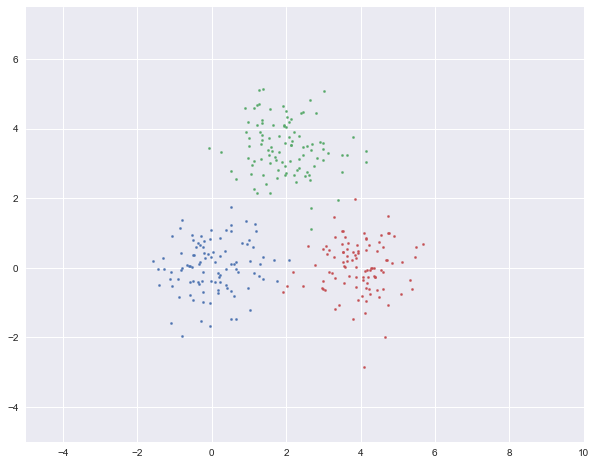
\includegraphics[width=.32\textwidth]{figure/1.1.png}
		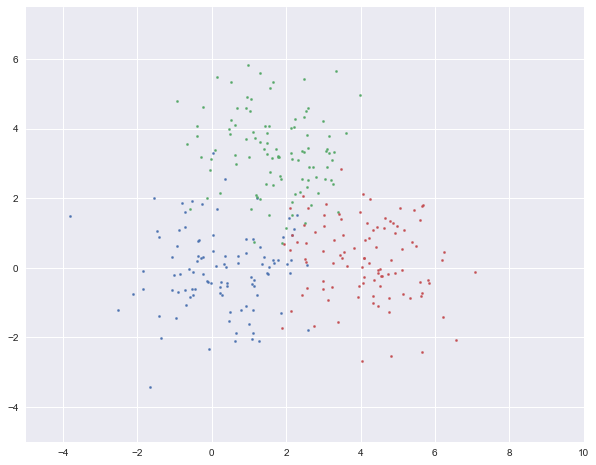
\includegraphics[width=.32\textwidth]{figure/1.2.png}
		\caption{代表性测试数据集}\label{f1}
	\end{figure}
	图\ref{f1}中,左边为标准差等于0.67是样本数据的分布,右边为标准差等于1.67时样本点的分布。可以看出数据集在标准差较小可以划分为明显的三个成分,在标准差变为所给的最大值时,已经看不出较为明显的聚类个数。
	
	加下来我将分别使用AIC准则、PC准则以及MML准则分别对样本数据进行定阶研究。图\ref{f2}为各个模型的估计结果。
	
	\begin{figure}[H]
		\centering
		% Requires \usepackage{graphicx}
		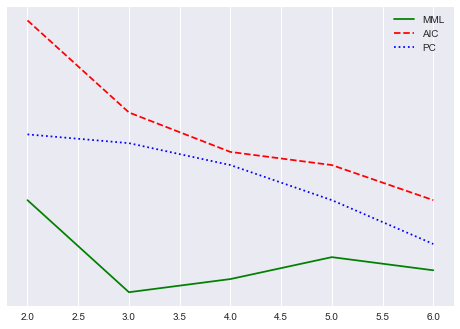
\includegraphics[width=140mm,height=90mm]{figure/1.3.png}\\
		\caption{估计结果}\label{f2}
	\end{figure}
	
	坐标轴横轴表示成分数,纵轴表示相应的信息准则值。由于最优成分数总是出现在相应信息准则的极大值或极小值处,因此在它们值的拐点处我们往往能得到正确的成分个数。图中展示了MML、AIC和PC和对应的成分数$k$的曲线,只有在$k=3$时,MML达到了其极小值,进而准确识别了正确的成分个数。
	虽然AIC和PC也对结果有一定的暗示,但是并没有具体识别出来。
	
	为了检验MML在更一般情况下的有效性,我会接着进行数值实验,所使用的模型还是本节提到的\ref{eq40},样本数量为100个,成分数$k$的取值为$2\leq k_i\leq 5$,均值、方差保持不变,初始化每个$\alpha_i=\frac{1}{3}$。
	
    表\ref{tab1},\ref{tab2},\ref{tab3}表示不同信息准则在不同标准差和成分数下识别出的正确样本点个数。

    \begin{table}[H]
    \centering
    \caption{2成分二维混合模型模拟结果}
    \label{tab1}
    \begin{tabular}{ccccccccc}
    \hline
    \multirow{3}{*}{标准差} & \multicolumn{8}{c}{成分个数$k$的分布}                                                   \\ \cline{2-9} 
                         & \multicolumn{3}{c}{MML} & \multicolumn{2}{c}{PC} & \multicolumn{3}{c}{AIC} \\ \cline{2-9} 
                         & 2            & 3   & 4  & 2              & 3     & 2            & 3   & 4  \\ \hline
    0.67                 & 82           & 14  & 4  & \textbf{86}    & 14    & 78           & 10  & 12 \\ \hline
    1.00                 & \textbf{65}  & 20  & 15 & 62             & 38    & 71           & 5   & 24 \\ \hline
    1.33                 & \textbf{44}  & 36  & 20 & 33             & 69    & 40           & 22  & 38 \\ \hline
    1.67                 & 42           & 20  & 38 & 45             & 54    & \textbf{73}  & 27  & -  \\ \hline
    \end{tabular}
    \end{table}    
    
    
    \begin{table}[H]
    \centering
    \caption{3成分二维混合模型模拟结果}
    \label{tab2}
    \begin{tabular}{cccccccccc}
    \hline
    \multirow{3}{*}{标准差} & \multicolumn{9}{c}{成分个数$k$的分布}                                                   \\ \cline{2-10} 
                         & \multicolumn{3}{c}{MML} & \multicolumn{3}{c}{PC} & \multicolumn{3}{c}{AIC} \\ \cline{2-10} 
                         & 2      & 3      & 4     & 2      & 3     & 4     & 3      & 4      & 5     \\ \hline
    0.67                 & 8      & 86     & 6     & 15     & 76    & 9     & \textbf{88}     & 10     & 2     \\ \hline
    1.00                 & 16     & \textbf{70}     & 14    & 55     & 34    & 11    & 10     & 66      & 24    \\ \hline
    1.33                 & 28     & \textbf{60}     & 12    & 47     & 33    & 20    & 22     & 55    & 23    \\ \hline
    1.67                 & 41     & \textbf{58}     & 1     & 68     & 32    & -     & 54     & 46     & -     \\ \hline
    \end{tabular}
    \end{table}
    

    \begin{table}[H]
    \centering
    \caption{4成分二维混合模型不同信息准则的识别结果}
    \label{tab3}
    \begin{tabular}{ccccccccc}
    \hline
    \multirow{3}{*}{标准差} & \multicolumn{8}{c}{成分个数$k$的分布}                                                   \\ \cline{2-9} 
                         & \multicolumn{3}{c}{MML} & \multicolumn{2}{c}{PC} & \multicolumn{3}{c}{AIC} \\ \cline{2-9} 
                         & 3   & 4            & 5  & 3     & 4              & 3      & 4      & 5     \\ \hline
    0.67                 & 15  & 85  & -  & 13    & \textbf{87}             & 7      & 81     & 12    \\ \hline
    1.00                 & 13  & \textbf{76}  & 11 & 63    & 37             & 24     & 5      & 71    \\ \hline
    1.33                 & 44  & \textbf{47}           & 9  & 69    & 33    & 8     & 40     & 52     \\ \hline
    1.67                 & 31  & \textbf{59}  & 20 & 38    & 62             & 43     & 38     & 19    \\ \hline
    \end{tabular}
    \end{table}
    
    如表\ref{tab1},\ref{tab2},\ref{tab3}所示,表的横轴表示相应信息准则以及被估计的成分(components)个数,纵轴表示不同的标准差。我们已经得知在标准差较小时高斯混合模型会有一个较为明显的聚集分布,随着标准差的增加,混合模型的分布会变得越来越集中,会更趋于一个整体。试验结果显示,在标准差较小时,MML、AIC、PC都能较好的识别出正确的成分个数。随着标准差的逐渐增大,三个信息准则的识别正确率都有所降低,但是相比于PC和AIC,MML还是明显更加可靠,特别是在分量密度基本重叠的情况下。AIC往往会高估正确的成分个数,而PC往往会低估正确的成分个数,这都与它们的惩罚函数有直接关联。
    
    经过生成数据的模拟,我们可以看到,相对来说,MML准则似乎是高斯混合模型成分选择时的最优准则,在低标准差时MML表现优秀,在高标准差时仍可以有着不错的准确率。相比与AIC、PC、MDL等准则,MML准则更加保守。
    
	接着我将会对MML-DAEM算法的聚类效果进行分析。所使用的模拟数据依然为本章开头所提到的高斯混合模型生成。不过成分个数变为四个以模拟更复杂的情况。为了使模拟结果更具说服力,生成数据时采用不平衡数据集的方式,各个成分分别生成80,100,120,100条数据。所生成的数据见图\ref{f3}:
	
	\begin{figure}[H]
	\centering
	% Requires \usepackage{graphicx}
	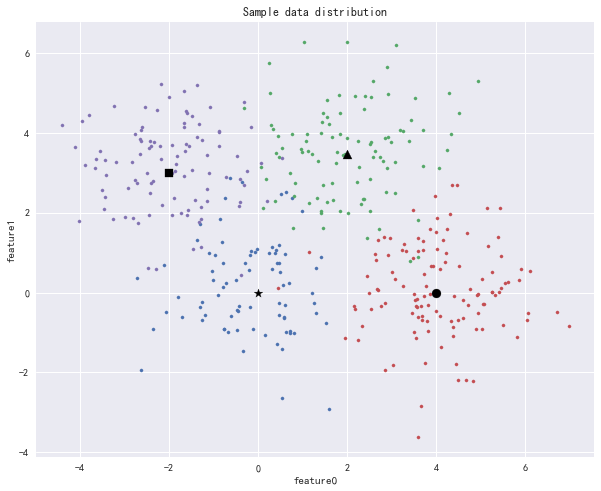
\includegraphics[width=140mm,height=90mm]{figure/1.4.png}\\
	\caption{估计结果}\label{f3}
    \end{figure}
    
	图\ref{f3}中为真实的样本数据,红色为第一类高斯分布生成数据,蓝色为第二类高斯分布所生成数据,绿色为第三类高斯分布所生成数据,紫色为第四类高斯分布生成的数据。黑色圆形点、黑色星形点、黑色三角形点、黑色矩形点分别表示第1、2、3、4类样本数据的均值向量,散点图坐标横轴表示第一维度,纵轴表示第二维度。
	
	接着本文将分别使用传统的EM算法、k-means聚类法以及所提出的MML-DAEM方法分别对模拟数据进行拟合分析。
	
	\begin{table}[H]  
		\centering
		\caption{高斯混合模型模拟研究中算法的模拟结果}
		\label{tab4}
		\medskip
		\begin{tabular}{c ccccccc}
			\hline  %p{1.2cm}
			& K-means & EM & MML-DAEM &\\
			\hline
			Step & 120.1 & 132.2 &210.3 &\\
			ACCURACY      & 0.8610 & 0.8625      & \textbf{0.9267}      &\\
			NMI          & 0.6375 & 0.6321    & \textbf{0.7824}     &\\
			ARI           & 0.6719         & 0.6795              & \textbf{0.8080}             &\\
            F值   &0.9252 &0.9424 &\textbf{0.9668} &\\
            Log-L &- &-4.401 &-4.207 &\\
			\hline
		\end{tabular}
		\begin{tablenotes}
			\footnotesize
			\item 注释: 表内所得到的数据均为多次模拟所得到的平均值。 Log-L表示对数似然函数大小。由于K-means算法不具有计算对数似然函数功能,其对应值为空。加粗的数字表明所对应列的算法估计效果最佳。
		\end{tablenotes}
	\end{table}
	
	\begin{table}[H]  
		\centering
		\caption{高斯混合模型模拟研究中算法的参数估计精度}
		\label{tab5}
		\medskip
		\begin{tabular}{c ccccccc}
			\hline  %p{1.2cm}
			& EM & C-EM & MML-DAEM &\\
			\hline
			
			$MAE(\hat{\alpha})$ & 0.059         & 0.042             & \textbf{0.023}              &\\
			$MAE(\hat{\mu})$    & 0.431        & 0.278              & \textbf{0.195}              &\\
			$MAE(\hat{\Sigma})$ & 0.616         & 0.332              & \textbf{0.302}              &\\
			\hline
		\end{tabular}
		\begin{tablenotes}
			\footnotesize
			\item 注释: 表内所得数据均为多次试验的平均值 $MAE(\hat{\theta})$记为各模型参数估计值与参数真值的平均绝对误差。 加粗的数字表明所对应列的算法估计效果最佳。
		\end{tablenotes}
	\end{table}
	

	
	
	由于本文所模拟试验生成的数据是认为是带有真实标签的,因此评价指标采用外部评价指标。表\ref{tab4}的第一列即为三种模型的各个评价指标, 依次为: 模型精确度Accuracy,标准互信息素NMI,调整兰德系数ARI,F值以及对数似然函数Log-L的大小。其中调整兰德系数ARI是兰德系数的一个改进版本,总的来说兰德系数是通过计算两个簇之间的相似度来对聚类结果进行评估。而调整兰德系数是对兰德系数基于几率正则化的一种改进。至于标准互信息素,本文之前也有提及,它也是基于互信息素的一种改进,总的来说互信息素也是用来衡量两种聚类结果(标签)之前相似程度的一个指标。
	
	本文所提出的MML-DAEM算法更多的是对获取最优成分数的改进,而模拟所使用的样本数据的聚类个数已经确定,因此在试验中便没有使用DAEM算法作为对照,并且试验更多的是对模型精度的探讨。
	在本文所做的模拟中,由于不是每一次模拟都能使得算法收敛,就算收敛也不一定得到有效的试验结果,因此为了得到更准确的模拟结果,本文对各个算法只采取符合预期的50次试验结果并取均值的计算方式。以下是对各个指标的详细讨论:
	
	\noindent(1) 聚类准确度方面, 本文所提出算法的平均聚类准确度最高, 传统的K-means聚类方法和EM算法相差无几。对比标准互信息素NMI和调整兰德系数ARI,同样是MML-DAEM方法有着更高的值,也就是有着更优异的模拟结果。
	
	\noindent(2) 从迭代次数方面分析, 传统的K-means方法和EM算法毫无疑问是有优势的,因为它们迭代初始值已经被设定为接近真实值的值,解决了EM算法最为不稳定因素之一,并且由于模型更简单具有更少的参数。 而不管是DAEM算法还是MML-DAEM算法, 都是在某个特定退火参数下进行迭代到收敛, 而每有一次退火参数的更新都会让EM算法重新进行迭代直到收敛。 因此所需要的迭代时间、空间复杂度通常会更高。
	
	\noindent(3) 对数似然函数值,由于K-means不具有对数似然函数,便没有进行对比。从结果来看,还是本文所提出的新方法具有更高的对数似然函数值。
	
	\noindent(4) 参数的平均绝对误差方面,总和对比均值、方差、混合比例系数可以发现 MML-DAEM方法的各参数的平均绝对误差更小,模型波动程度更小,也就是模拟结果更接近真实情况。
	
	各个模型模拟结果的图见图\ref{f4}、图\ref{f5}、图\ref{f6}.
	
	
	\begin{figure}[H]
	\centering
	% Requires \usepackage{graphicx}
	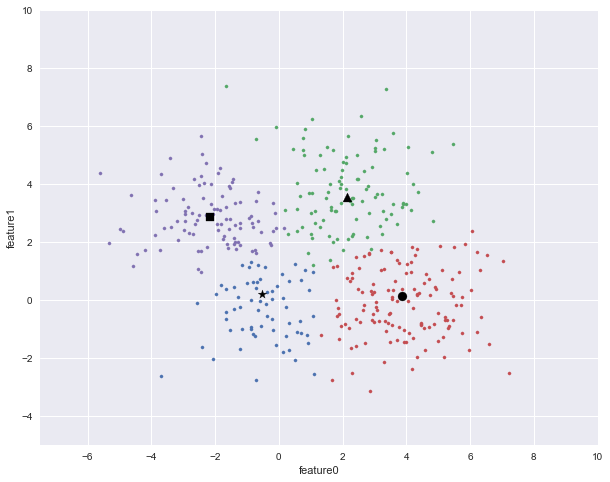
\includegraphics[width=140mm,height=90mm]{figure/1.7.png}\\
	\caption{EM模拟结果}\label{f4}
    \end{figure}
    
    	\begin{figure}[H]
	\centering
	% Requires \usepackage{graphicx}
	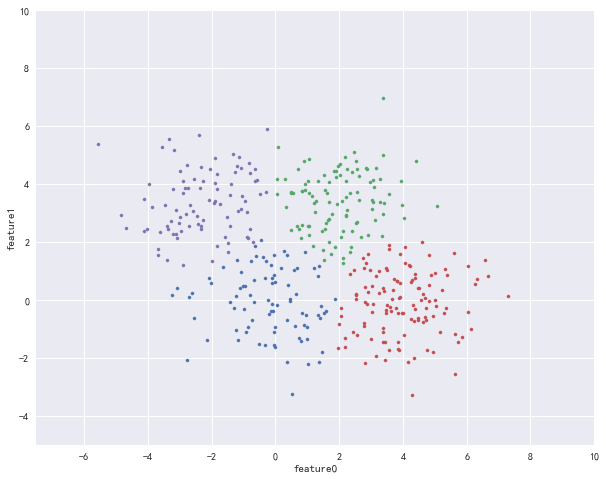
\includegraphics[width=140mm,height=90mm]{figure/1.6.png}\\
	\caption{K-means算法模拟结果}\label{f5}
    \end{figure}
    
    	\begin{figure}[H]
	\centering
	% Requires \usepackage{graphicx}
	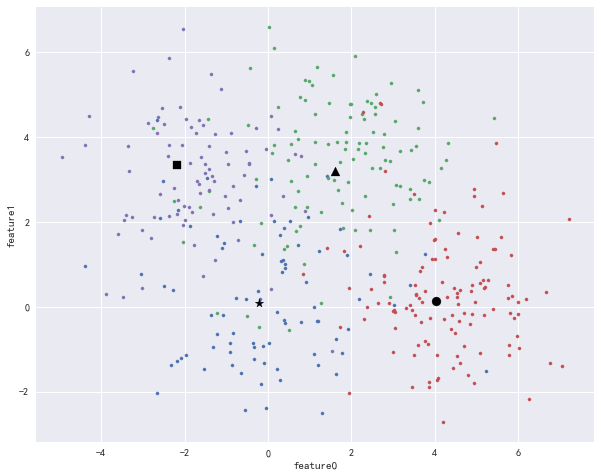
\includegraphics[width=140mm,height=90mm]{figure/1.5.png}\\
	\caption{MML-DAEM估计结果}\label{f6}
    \end{figure}
    
	图\ref{f4},\ref{f5},\ref{f6}分别为EM算法模拟结果,K-means模拟结果以及MML-DAEM模拟结果。K-means方法由于没有进行参数估计,因此没有画出聚类中心。从图中可以看出,三种方法能明显做出正确的聚类划分,都可以将样本数据分为四个类别。但是在细节上三种方法还是有不同之处。K-means方法在进行聚类划分时得出的结果更加”紧凑“,并且有非常明显的聚集特性;EM方法所模拟划分的数据在有明显聚类中心的情况下则变得相对分散;而MML-DAEM方法所模拟划分的数据最为分散,不仅如此,在划分的每个类别中都有零星的其他类别的数据点穿插其中,更加真实的模拟了样本数据的分布情况,因此带来了更高的精确度。
	
	总的来说,模拟研究结果表明在所给样本具有明显聚集分布时,也就是样本方差较小时,本文所提出算法和传统聚类方法都能较好识别出正确的成分个数以及聚类结果,但在样本标准差较大时就体现出来本文所提算法的优越性,无论从精确度还是其他评价指标来看,MML-DAEM方法都取得了更好的结果,唯一美中不足的是它的迭代时间稍长,接下来的研究中考虑对其进行进一步优化。
	
	
	\section{实证分析}
	本节将对一系列的真实复杂网络进行划分,从而验证所提MML-DAEM算法的合理性。所使用的数据集均是复杂网络的经典数据集,包括空手道俱乐部网络数据集、美国足球队数据集。
	
	\subsection{空手道俱乐部网络}
	这是著名的和经常使用的扎卡里空手道俱乐部网络数据。这些数据是由Wayne Zachary于1977年从一所大学空手道俱乐部的成员那里收集的。34个节点代表俱乐部的34名成员,两个节点之间的连边代表着对应着的两个成员有着密切的关系。网络是无方向的。使用该数据集经常讨论的一个问题是找到空手道俱乐部在两名教练发生争执后分裂成的两组人。
	
	图\ref{f7}是Zarchary俱乐部为划分前的复杂网络图,图\ref{f8}是Zarchary俱乐部节点的概率分布图,图\ref{f9}是经过本文所提出算法计算后得到的社区图。
	
	\begin{figure}[H]
	\centering
	% Requires \usepackage{graphicx}
	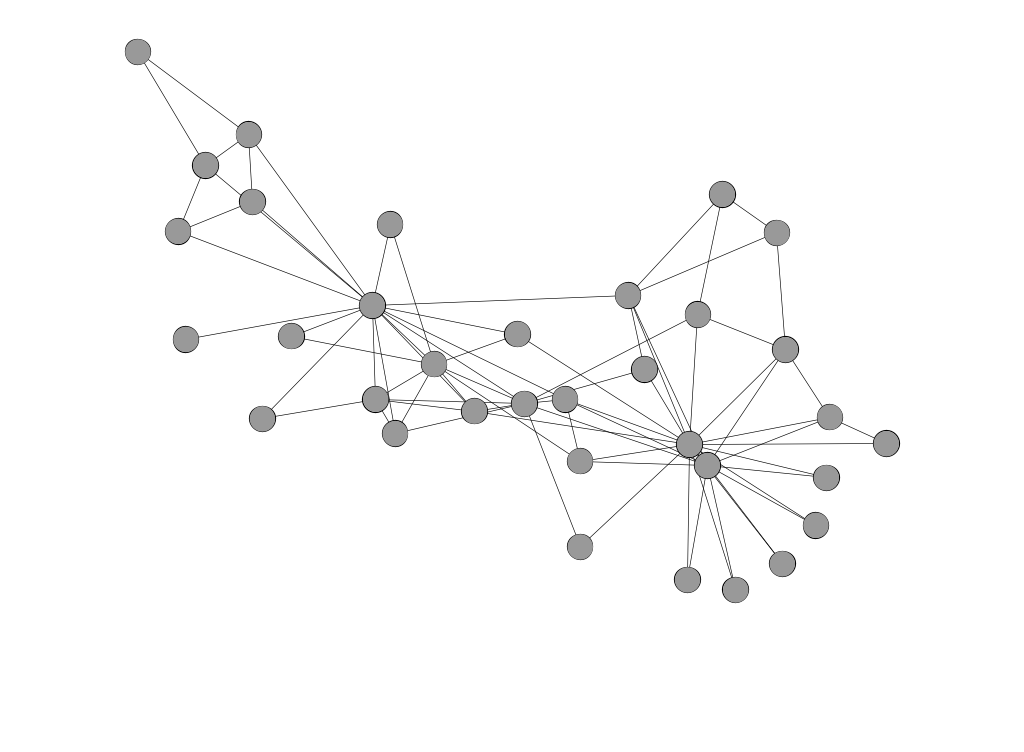
\includegraphics[width=120mm,height=90mm]{figure/karate-ori.png}\\
	\caption{Zachary空手道俱乐部}\label{f7}
    \end{figure}
    
	图\ref{f7}是未经划分原始复杂网络图,从中可以看到其节点及连边的连接关系以及节点的分布情况。图中可以看出有较为明显的社团分布,但是具体社团数目以及划分方法还要依赖下一步的计算分析。
	
	\begin{figure}[H]
	\centering
	% Requires \usepackage{graphicx}
	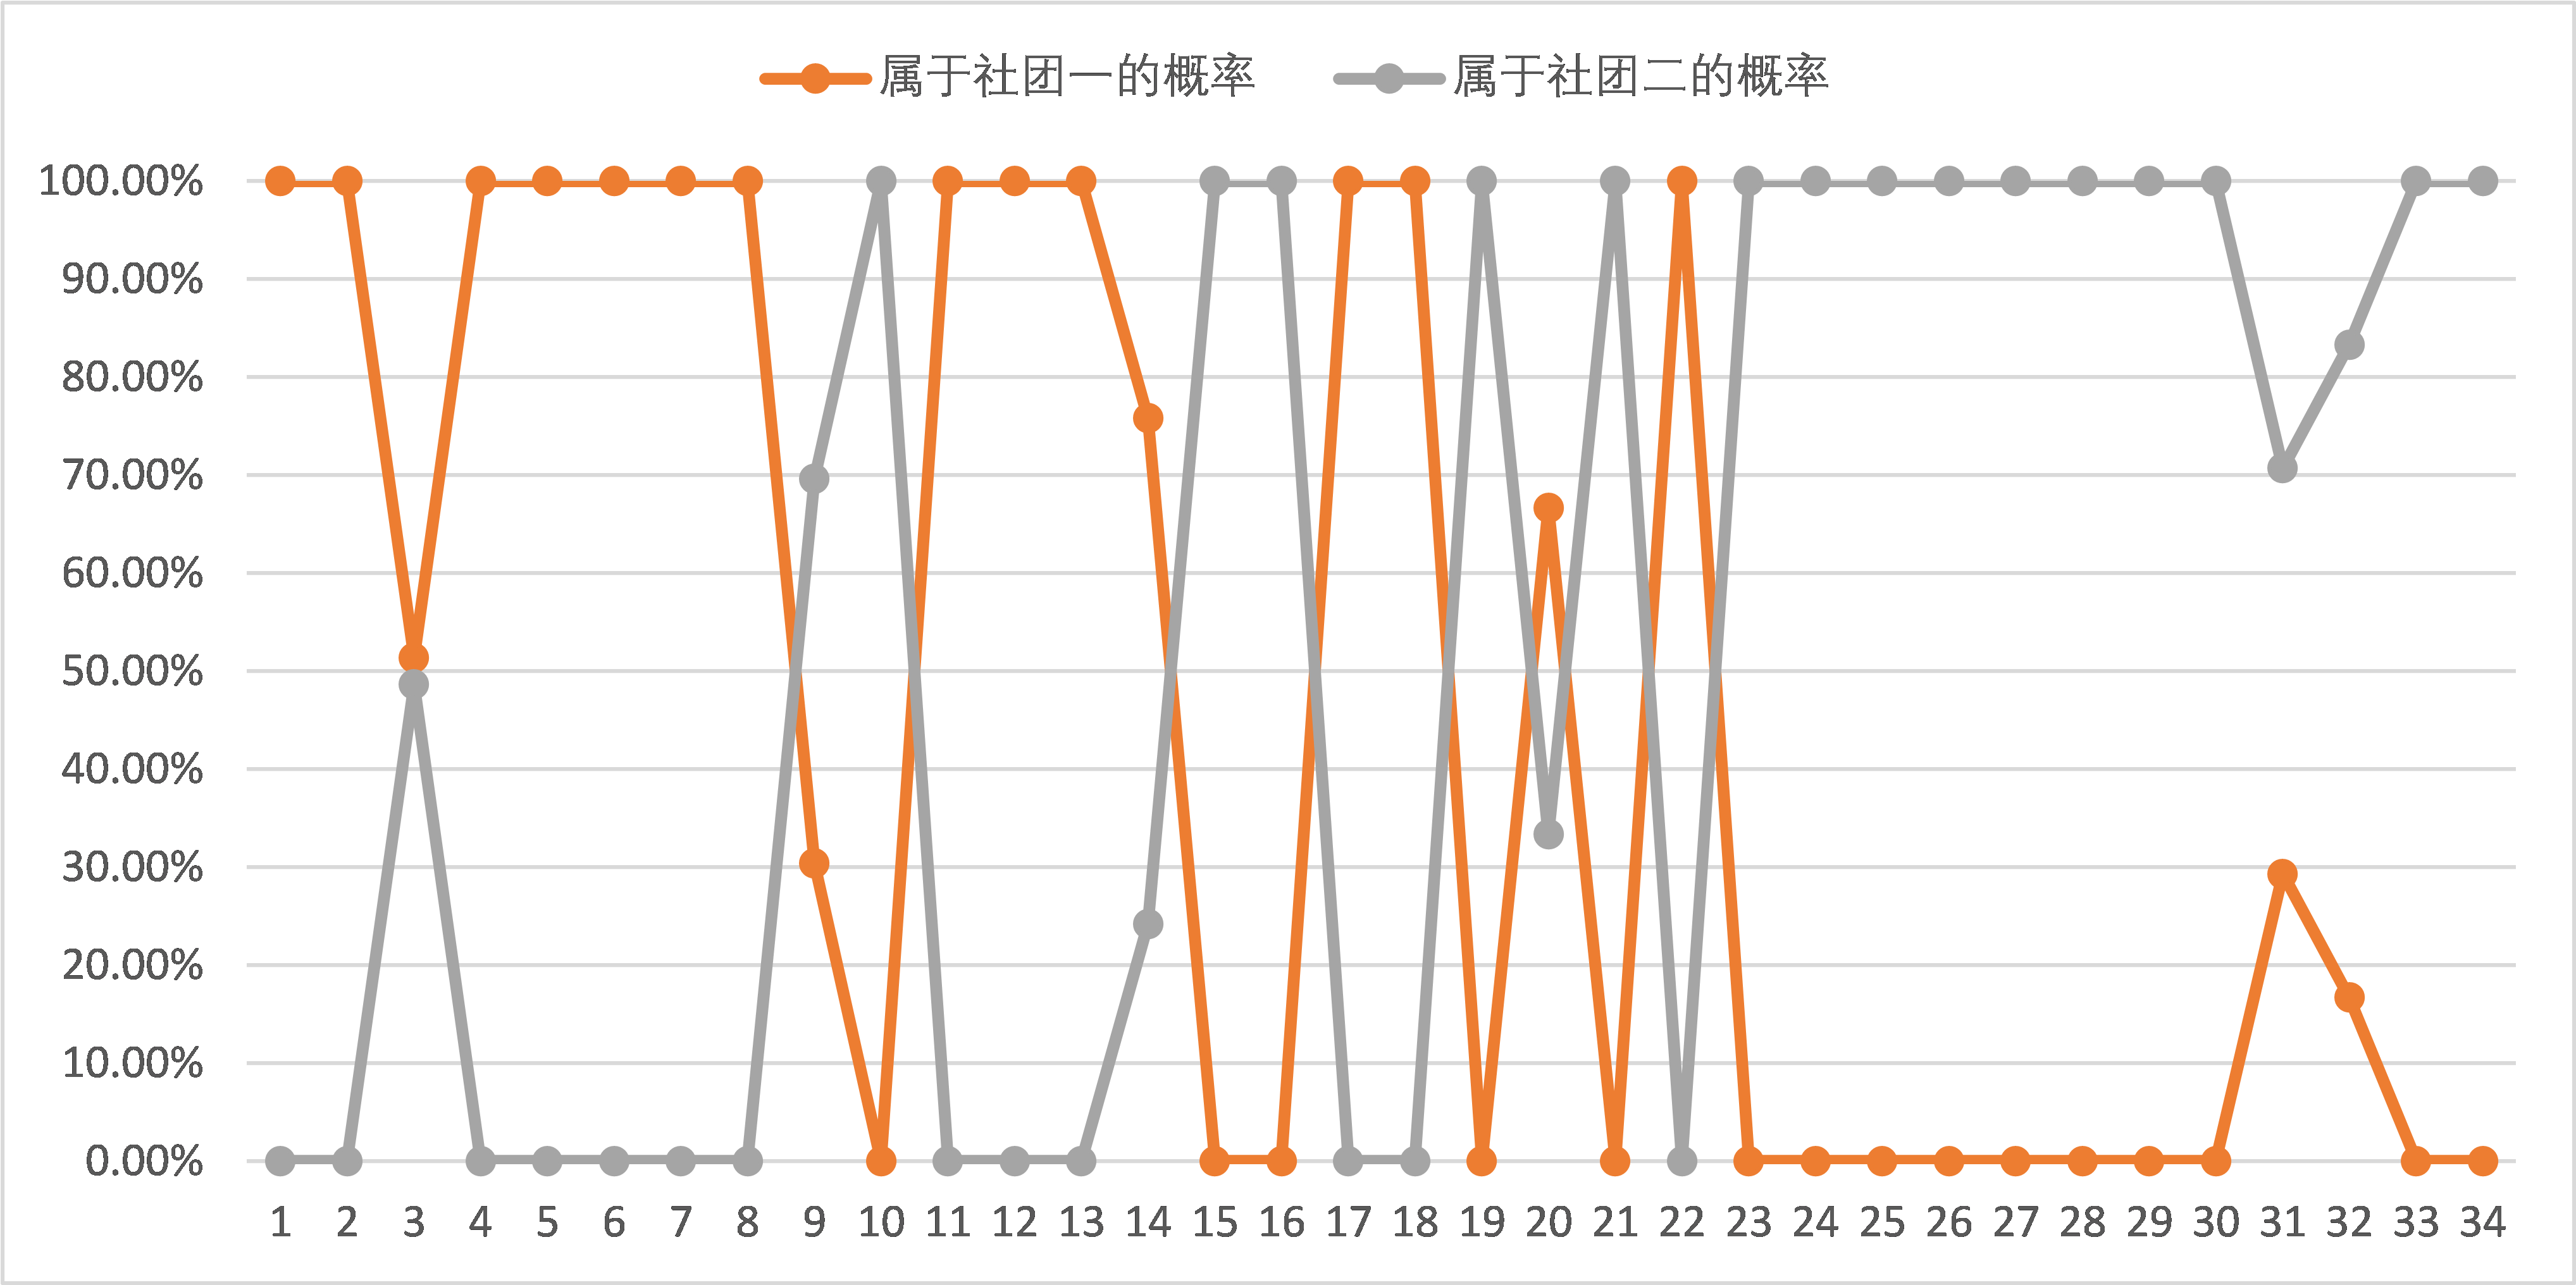
\includegraphics[width=140mm,height=80mm]{figure/karate-pro.png}\\
	\caption{Zachary空手道俱乐部节点概率分布}\label{f8}
    \end{figure}
	
	图\ref{f8}是经过MML-DAEM方法迭代计算过后的节点的概率分布图。横坐标表示Zachary俱乐部34个成员对应的34个节点,纵坐标表示相应节点对应的概率值,分别给出了每个节点所属每个社团的概率大小。从图中可以看到大部分节点的概率值分布在1和0两个值之中,即表明其已被完全划分到相应的社团之中。还有部分节点的概率值分布在0和1之间,则划分社团时要根据其值的大小进行进一步分析。
	
	\begin{figure}[H]
	\centering
	% Requires \usepackage{graphicx}
	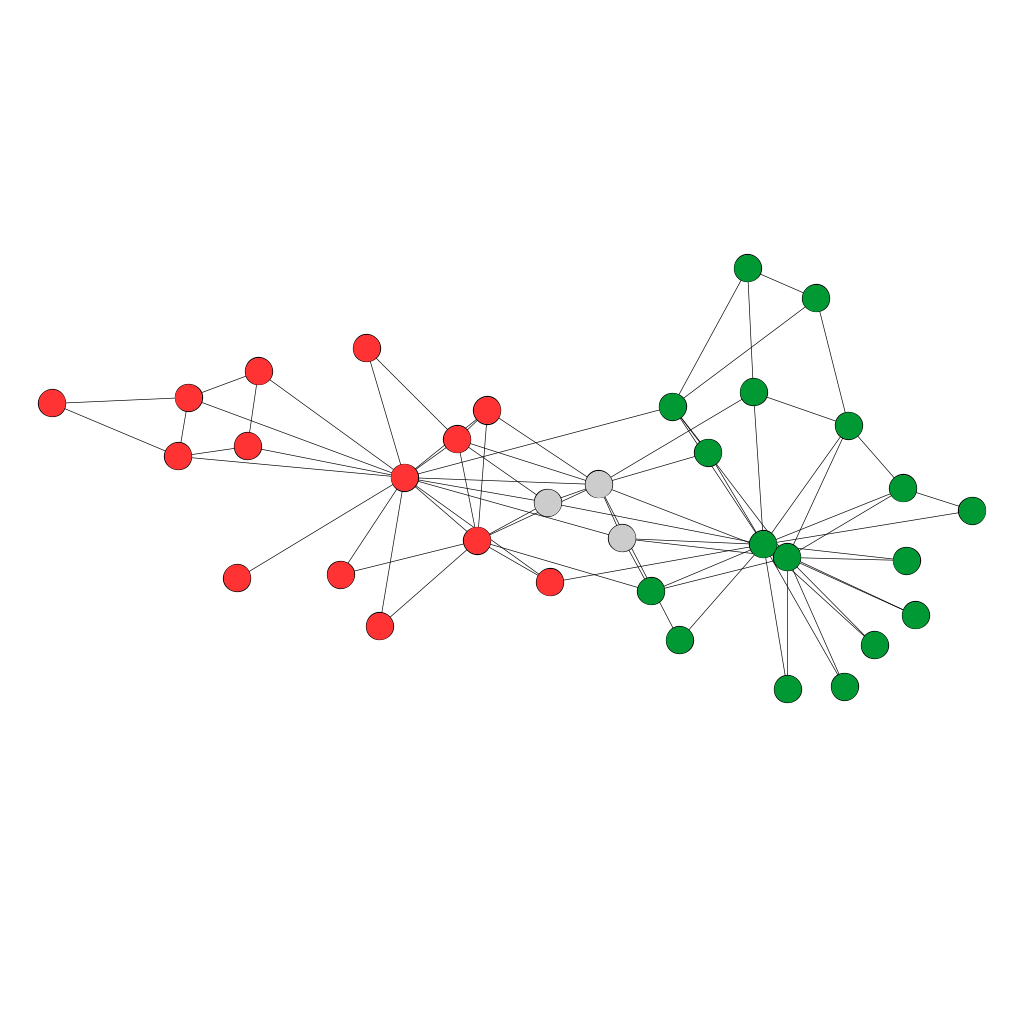
\includegraphics[width=110mm,height=110mm]{figure/karate.png}\\
	\caption{Zachary空手道俱乐部划分结果}\label{f9}
    \end{figure}
    
    图\ref{f9}表示Zachary空手道俱乐部最终的社团划分结果。经过本文所提出MML-DAEM方法迭代计算后,Zachary空手道俱乐部已被划分为两个较为明显的社区,分别使用红色节点和绿色节点标注,这个划分结果与实际情况十分相似。图中灰色节点表示有争议的部分,本文只将节点概率分布大于0.7的划分到相应社区,其他不满足条件的节点则使用灰色进行表示。其实在Zachary空手道俱乐部中,有一些成员在两个社区都有朋友,因此无论将他们划分到哪一个社区都会有困难,这也与本文的试验结果相符。
    
    然而,该算法揭示了更多关于网络的信息。由于生成模型的特殊性,算法的划分结果不再是简单的硬划分,即给出每个节点对应的社区,而是给出了每个节点所属社区的概率值,然后根据概率值的大小取判断该节点所属的实际社区。其实在实际情况中,有些节点并不是可以确切的划分到某个社区中,因为它既可以同时属于多个社区,也可以孤零零地存在。
    
    接着让我们来看看另一个更复杂试验的结果。
	\subsection{足球俱乐部网络}
	
	足球俱乐部网络是由Newman和其搭档Girvan构建而成。在该网络中共有115个节点表示115个参加美国足球赛的高校球队,节点之间的连边代表着对应的两支球队之间进行过比赛。足球俱乐部网络的社区则代表着足球俱乐部所属的联盟。
	
		
	\begin{figure}[H]
	\centering
	% Requires \usepackage{graphicx}
	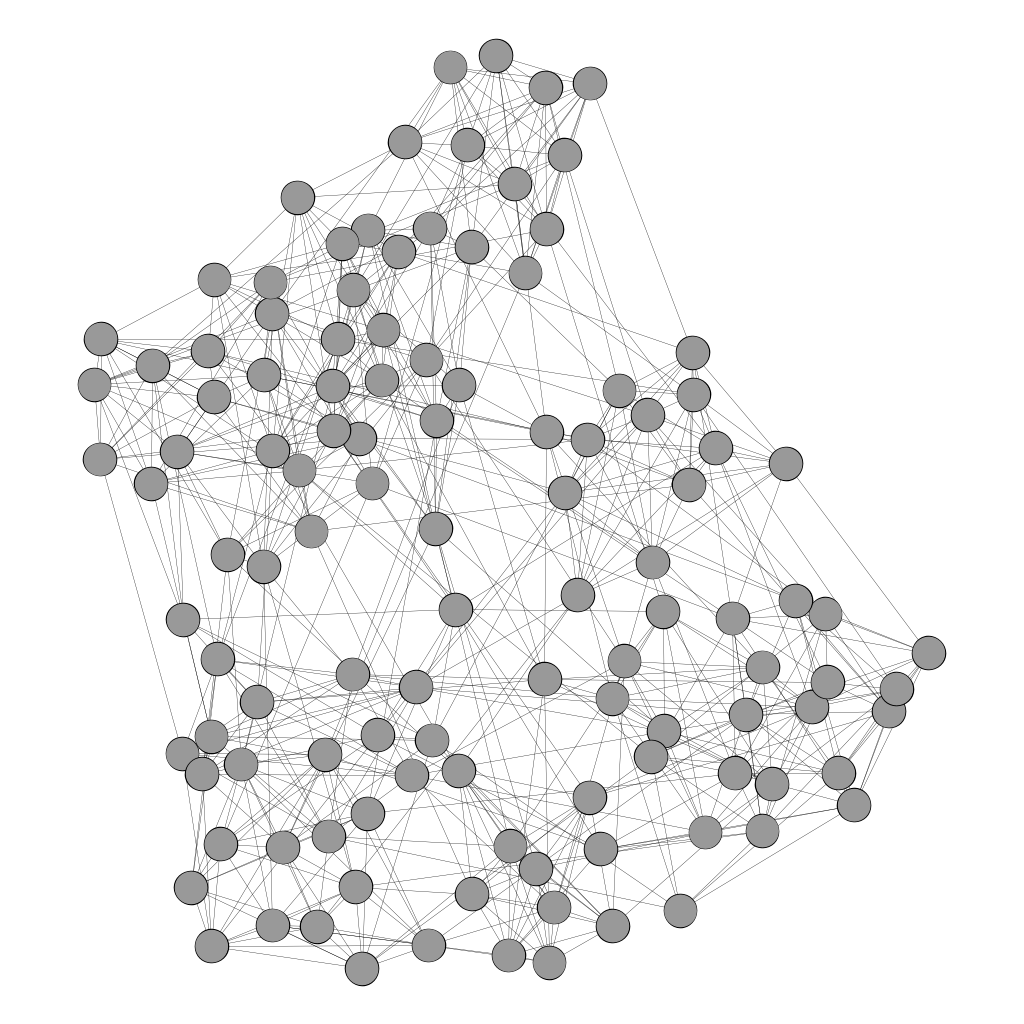
\includegraphics[width=100mm,height=100mm]{figure/football-ori.png}\\
	\caption{足球俱乐部网络}\label{f10}
    \end{figure}
	
	图片\ref{f10}为未经划分的足球俱乐部复杂网络图。可以明显看出足球俱乐部网络的分布情况要复杂的多,不仅顶点之间分布更密集,而且出现了社区重叠的现象,这无疑给我们的社区划分增加了难度。
	
	\begin{figure}[H]
	\centering
	% Requires \usepackage{graphicx}
	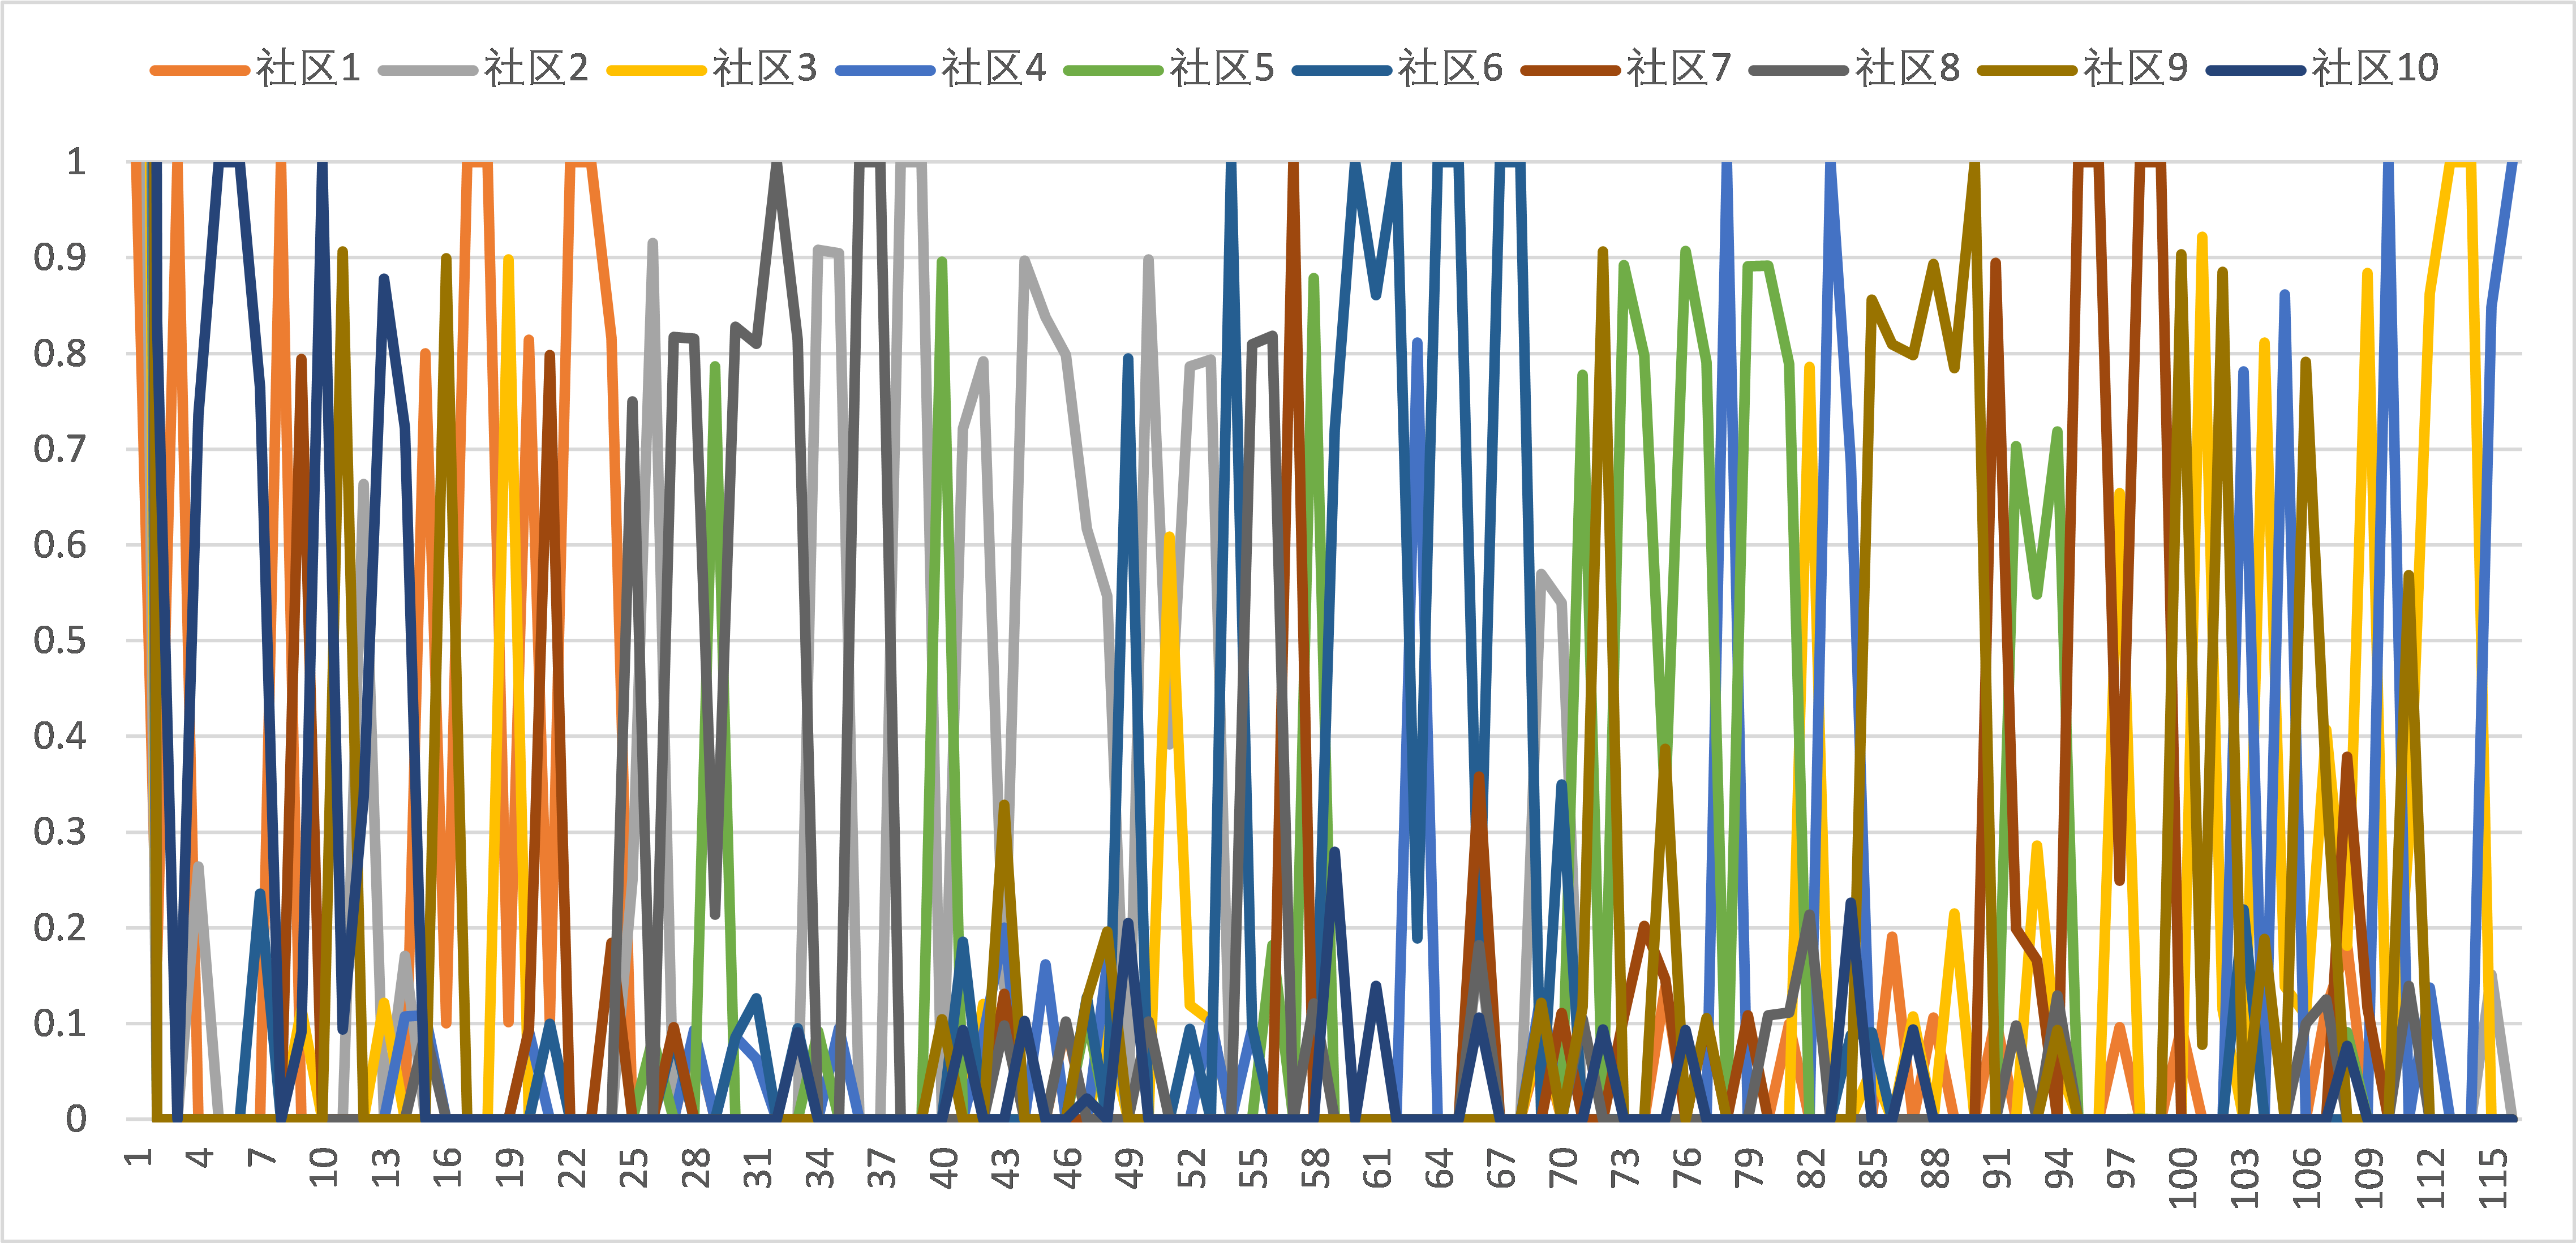
\includegraphics[width=160mm,height=70mm]{figure/football-pro.png}\\
	\caption{足球俱乐部网络节点概率分布}\label{f11}
    \end{figure}
	
	\begin{figure}[H]
	\centering
	% Requires \usepackage{graphicx}
	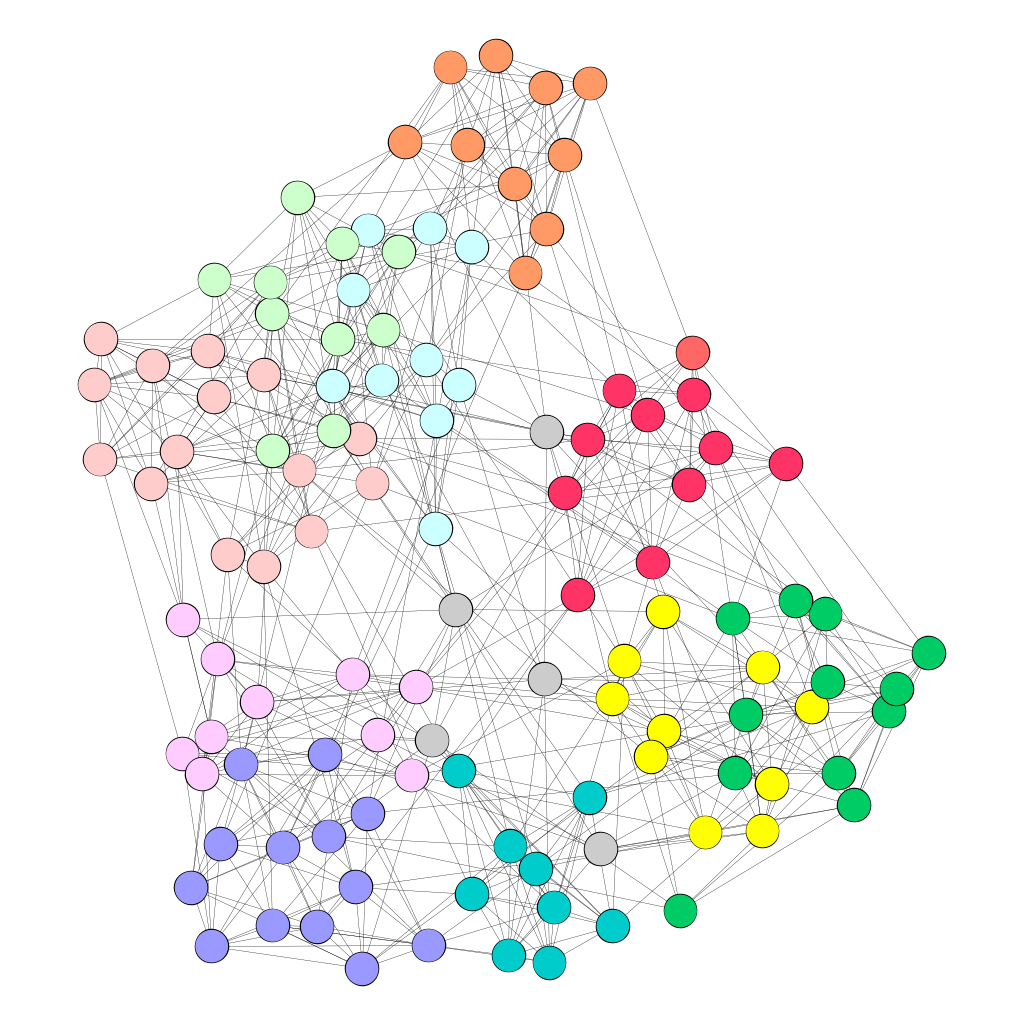
\includegraphics[width=100mm,height=100mm]{figure/football.png}\\
	\caption{足球俱乐部网络划分结果}\label{f12}
    \end{figure}
	
	图\ref{f11},图\ref{f12}分别为足球俱乐部网络节点概率分布图和足球俱乐部网络的划分结果。
	
	图\ref{f11}表明115个足球俱乐部共有10个足球联盟,并给出了每个足球队所属足球联盟的概率,并且多数概率值都在0.7-1之间,表明相应足球队有大概率属于对应的足球联盟。
	
	图\ref{f12}为足球俱乐部网络最终的划分结果,不同颜色表示不同的足球联盟。不同于Zachary空手道俱乐部的划分方式,由于足球俱乐部联盟众多,因此本文将足球俱乐部所属联盟的概率是否大于0.5为标准,大于0.5时将对应俱乐部划分到相应的联盟内,小于0.5则将其标注为灰色,表明其划分存在争议。从图中可以看出大部分足球俱乐部都得到了划分,只有5个足球俱乐部难以判别。
	当顶点集中重叠在一起时,复杂网络的社团提取效果往往很难达到预期,比如图中的左上角和右下角区域,顶点重叠区域一直是复杂网络社团提取的难点。但本文所提出的方法在计算重叠部分时算得上是差强人意。
	
	接着我将比较MML-DAEM方法和GN\cite{ref8}算法在Zachary空手道俱乐部网络、足球俱乐部网络、海豚社交网络上的模块度Q和标准互信息素NMI的大小。
	
	\begin{table}[H]
	\centering
	\caption{四个不同网络试验结果}
	\label{t6}
    \begin{tabular}{ccccc}
    \hline
    \multirow{2}{*}{Networks} & \multicolumn{2}{c}{Avg Q} & \multicolumn{2}{c}{Avg NMI} \\ \cline{2-5} 
                              & GN         & MMl-DAEM     & GN          & MML-DAEM      \\ \hline
    Zachary Karate club       & 0.2551     & 0.3557       & 0.8107      & 0.8372        \\ \hline
    Dolphin's Social Network  & 0.3102     & 0.2711       & 0.7210      & 0.6913        \\ \hline
    Moreno Lesmis             & 0.3041     & 0.3345       & 0.6887      & 0.7211        \\ \hline
    American College football & 0.2374     & 0.2410       & 0.5021      & 0.5101        \\ \hline
    \end{tabular}
    \end{table}
	
	表\ref{t6}为传统GN算法和MML-DAEM方法在四个不同真实网络上的试验结果。试验结果的好坏由平均模块度Q和平均标准互信息素共同决定。每个算法均进行了20次独立试验。对于Zachary空手道俱乐部,悲惨世界任务关系网以及足球俱乐部网络,MML-DAEM方法的的均优于GN算法;只有海豚网络GN算法的Q和NMI略高于本文所提方法。总的来说,MML-DAEM方法以及取得了很不错的试验结果。
	
	下图为四个不同复杂网络的Q和NMI箱线图。
	
	这些箱线图为20次独立运行的统计结果,主要用于分析数据内部的分散状态或分布状态,包括数据上限、下限、上四分位数、下四分位数、中位数、异常值等。
	\begin{figure}[htp]
    \centering
    \begin{minipage}[t]{0.49\textwidth}
        \centering
        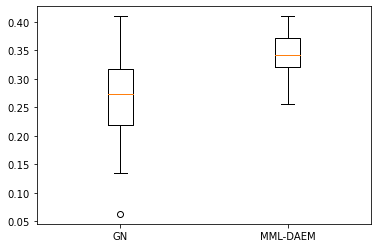
\includegraphics[width=1\textwidth]{figure/karate-q.png}
        \caption{Karate club - Q}
        \label{f13}
    \end{minipage}
    \begin{minipage}[t]{0.49\textwidth}
        \centering
        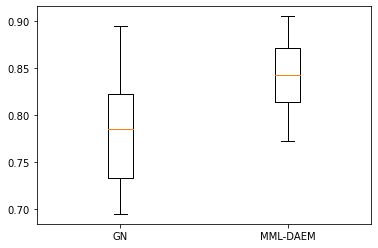
\includegraphics[width=1\textwidth]{figure/karate-nmi.png}
        \caption{Karate club - NMI}
        \label{f14}
        \end{minipage}
    \end{figure}
    
    \begin{figure}[htp]
    \centering
    \begin{minipage}[t]{0.49\textwidth}
        \centering
        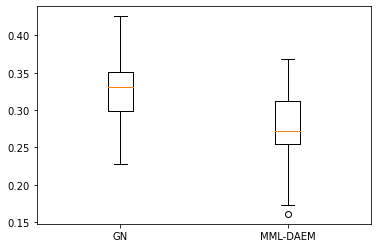
\includegraphics[width=1\textwidth]{figure/dolphin-q.png}
        \caption{Dolphin's social - Q}
        \label{f15}
    \end{minipage}
    \begin{minipage}[t]{0.49\textwidth}
        \centering
        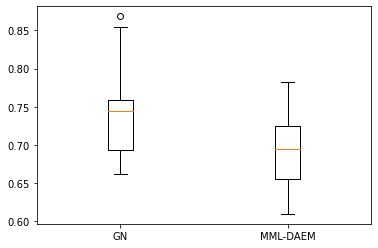
\includegraphics[width=1\textwidth]{figure/dolphin-nmi.png}
        \caption{Dolphin's social - NMI}
        \label{f16}
        \end{minipage}
    \end{figure}
    
    \begin{figure}[htp]
    \centering
    \begin{minipage}[t]{0.49\textwidth}
        \centering
        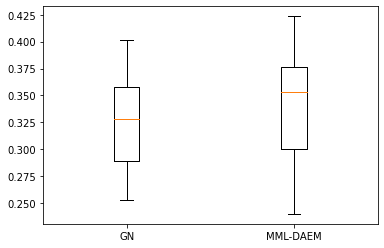
\includegraphics[width=1\textwidth]{figure/moreno-q.png}
        \caption{Moreno lesmis - Q}
        \label{f17}
    \end{minipage}
    \begin{minipage}[t]{0.49\textwidth}
        \centering
        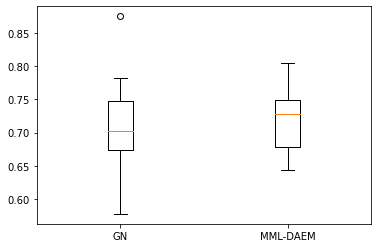
\includegraphics[width=1\textwidth]{figure/moremo-nmi.png}
        \caption{Moreno lesmis - NMI}
        \label{f18}
        \end{minipage}
    \end{figure}
	
	\begin{figure}[htp]
    \centering
    \begin{minipage}[t]{0.49\textwidth}
        \centering
        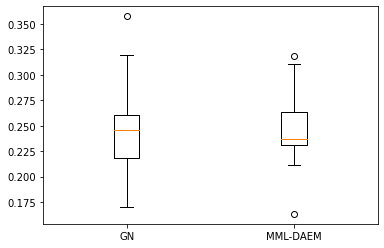
\includegraphics[width=1\textwidth]{figure/football-q.png}
        \caption{Football - Q}
        \label{f19}
    \end{minipage}
    \begin{minipage}[t]{0.49\textwidth}
        \centering
        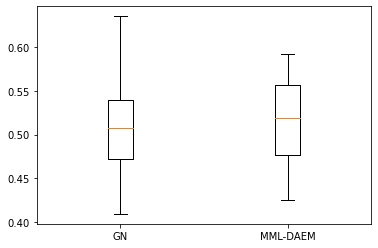
\includegraphics[width=1\textwidth]{figure/football-nmi.png}
        \caption{Football - NMI}
        \label{f20}
        \end{minipage}
    \end{figure}
    图\ref{f13},\ref{f14}为Zachary空手道俱乐部网络的20次独立计算结果。可以看出,相比于GN算法,MML-DAEM方法计算得到的模块度Q值和标准互信息素NMI总体来说更大,并且其值Q值和NMI值的分布更集中,MML-DAEM方法取得了更好的试验结果。
    
    图\ref{f15},图\ref{f16}为海豚网络的模拟结果,总的来说GN方法和MML-DAEM方法差别不是太大,但是GN方法还是有一些优势,主要是由于海豚网络不同于其他网络,它的社区结构因为海豚群居习性的关系更加紧密。
    
    图\ref{f17},图\ref{f18}为悲惨世界人物关系网的试验结果,可以看出GN方法和MML-DAEM方法所得结果差别也不是很大,但是MML-DAEM方法数据更集中,异常值也较少,有着更高的上四分位数和上界,总体来说MML-DAEM方法还是优于GN方法。
    
    图\ref{f19},图\ref{f20}为美国足球网络试验结果。从图中可以看出GN方法所得结果具有较多异常值,并且其数据分布更广泛,而MML-DAEM方法则表现得更好,不仅数据分布集中,而且其Q和NMI更高。
    
    
	\chapter[总结与展望]{总结与展望}\fancyhead[C]{\xiaowuhao}
	\section{总结}
	在现实生活中,不论是高斯混合模型还是EM算法还是复杂网络,它们都有着深刻的理论基础与广泛的应用。一提到高斯混合模型,离不开的就是参数估计问题,随之而来的就是EM算法,但是由于EM算法其本身局限性,Ueda\cite{ref21}给出了其解决方案。本文就是在Ueda等人提出的关于退火参数理论基础上提出了MML-DAEM方法,用于解决模型定阶和参数估计问题。
	
	MML-DAEM方法是一种迭代算法,不仅适用于混合模型,也同样适用于复杂网络。数值模拟和真实数据试验证明本文所提出的MML-DAEM方法在收敛性和聚类准确度方面都取得了很好的结果。传统的复杂网络社团提取方法在面对社团重叠问题、顶点模糊问题时往往束手无策,但是本文所提方法是一种基于概率统计的生成模型,它可以确切地给出每个顶点所属社团的概率,而不再是简单的0-1问题,这无疑给我们的判断带来了极大的方便。
	
	本文所做的研究均是站在巨人的肩膀上才得以顺利进行。尤其时M E J Newman、Grivan、Ueda等著名学者的研究结果给本人提供了丰富的学习经验。
	
	\section{未来的工作}
	下面总结以下本文研究不足之处以及未来的研究工作。主要研究内容包括算法进一步优化问题,其他分布的参数估计问题以及复杂网络方面的进一步优化研究等。
	
	
	\subsection{算法优化问题}
	确定性退火方法虽说使用与解决EM算法收敛到局部最大值问题,但是在某些情况下并不能保证其能够收敛到全局最大值,比如当似然函数的两个极值点距离过远。还有一个问题是算法的收敛时间略长。由于对每一个退火参数$\beta$,MML-DAEM方法都要进行一次完整的直到收敛的迭代,因此整个算法的计算时间是比EM算法要长的,在数据量大时尤为明显。其优化问题将一直会是接下来研究的重点。
	\subsection{其他类型数据的参数估计问题}
	本文所提方法是一种迭代方法,目前只应用在了高斯混合模型和复杂网络上。
	本文主要研究的是高斯混合模型和复杂网络的参数估计问题,但是还有其他混合模型,比如泊松混合模型、二项混合模型等也同样具有研究价值。异质混合模型及含有不同成分的混合模型同样可以进行研究。
	
	\subsection{复杂网络方面}
	本文所研究的真实复杂网络均是小型无向复杂网络,在面对超大型复杂网络时比如电力网络、Email网络等具有成千上万个节点和社团的数据时本文所提方法是否还能有效验证仍然未知,这还需要进行进一步的研究。
	
	
	
	
	
	\bibliography{bibliography}
	
	%%%%%%%%%%%%%%%%%%%%%%%%%%%%%%%%%%%%%%%%%%%%%%%%%%%%%%%%%%% 参考文献
	\newpage
	\pagestyle{fancy}
	\begin{spacing}{1.2}
		\begin{thebibliography}{1}\wuhao{
            \bibitem{ref1}
            Chialvo D R.
            \newblock Critical brain networks[J].
            \newblock {Physica A: Statistical Mechanics and its Applications}, {
              2004}, {340(4)}: {756-765}.
            
            \bibitem{ref2}
            Watts D J, Strogatz S H. 
            \newblock Collective dynamics of ‘small-world’networks[J].
            \newblock {Nature} ,{ 1998}, {393(6684):440-442}.
            
            \bibitem{ref3}
            BarabasiAL, Albert R.
            \newblock Emergence of scaling in random networks[J].
            \newblock {Science},1999,286(5439):509--512.
            
            \bibitem{ref4}
            Windham M P, Cutler A.
            \newblock Information ratios for validating mixture analyses[J].
            \newblock {Journal of the American Statistical Association} ,{ 1992, 87(420):1188-1192}.
            
            \bibitem{ref5}
            Girvan M, Newman M E J.
            \newblock Community structure in social and biological networks[J].
            \newblock { Proceedings of the national academy of sciences}, { 2002,99(12):7821-7826}.
            
            \bibitem{ref6}
            Donetti L, Munoz M A. 
            \newblock Detecting network communities: a new systematic and efficient
              algorithm[J].
            \newblock {Journal of Statistical Mechanics: Theory and Experiment},{
              2004,2004(10)P10012}.
              
            \bibitem{ref7}
            Reichardt J, Bornholdt S.
            \newblock Detecting fuzzy community structures in complex networks with a Potts
              model[J].
            \newblock { Physical review letters},{ 2004,93(21):218701}.
            
            \bibitem{ref8}
            Pons P, Latapy M.
            \newblock Computing communities in large networks using random walks[C].
            \newblock In Proceedings of the International symposium on computer and
              information sciences. Springer, 2005:284--293.
            
            \bibitem{ref9}
            Wu F, Huberman B A.
            \newblock Finding communities in linear time: a physics approach[J].
            \newblock {The European Physical Journal B} ,{ 2004}, { 38(2):331-338}.
            
            \bibitem{ref10}
            Duch J, Arenas A. 
            \newblock Community detection in complex networks using extremal optimization[J].
            \newblock {Physical review E},{ 2005,72(2):027104}.
            
            \bibitem{ref11}
            Newman M E J.
            \newblock Fast algorithm for detecting community structure in networks[J].
            \newblock {Physical review E},{ 2004,69(6):066133}.
            
            \bibitem{ref12}
           Guimera R, Sales-Pardo M, Amaral L A N.
            \newblock Modularity from fluctuations in random graphs and complex networks[J].
            \newblock {Physical Review E},{ 2004,70(2):025101}.
            
            \bibitem{ref13}
            Newman M E J, Leicht E A. 
            \newblock Mixture models and exploratory analysis in networks[J].
            \newblock {Proceedings of the National Academy of Sciences},{ 2007,
              104(23):9564-9569}.
              
            \bibitem{ref14}
            Wang X F.
            \newblock Complex networks: topology, dynamics and synchronization[J].
            \newblock {International journal of bifurcation and chaos},{ 2002,12(05):885-916}.
            
            \bibitem{ref15}
            朱涵,王欣然,朱建阳.
            \newblock 网络 “建筑学”[J].
            \newblock {物理},{2003,32(06):0-0}.
            
            \bibitem{ref16}
            吴金闪,狄增如.
            \newblock 从统计物理学看复杂网络研究[J].
            \newblock {物理学进展},{ 2004,24(1):18-46}.
            
            \bibitem{ref17}
            刘涛,陈忠,陈晓荣.
            \newblock 复杂网络理论及其应用研究概述[J].
            \newblock {系统工程},{2005,23(6):1-7}.
            
            \bibitem{ref18}
            史定华.
            \newblock 网络——探索复杂性的新途径[J].
            \newblock {系统工程学报},{2005}, {20(2):115-119}.
            
            \bibitem{ref19}
            Newman M E J.
            \newblock Detecting community structure in networks[J].
            \newblock {The European physical journal B},{ 2004, 38(2):321-330}.
            
            \bibitem{ref20}
            Newman M E J,Girvan M.
            \newblock Finding and evaluating community structure in networks[J].
            \newblock {Physical review E},{ 2004,69(2):026113}.
            
            \bibitem{ref21}
            Dempster A P, Laird N M, Rubin D B. 
            \newblock Maximum likelihood from incomplete data via the EM algorithm[J].
            \newblock {Journal of the Royal Statistical Society: Series B
              (Methodological)},{1977,39(1):1-22}.
            
            \bibitem{ref22}
            Ueda N, Nakano R. 
            \newblock Deterministic annealing EM algorithm[J].
            \newblock {Neural networks},{ 1998, 11(2):271-282}.
            
            \bibitem{ref23}
            Wolfe J H.
            \newblock Pattern clustering by multivariate mixture analysis[J].
            \newblock {Multivariate behavioral research},{ 1970,  5(3):329-350}.
            
            \bibitem{ref24}
            Jaynes E T.
            \newblock Information theory and statistical mechanics[J].
            \newblock {Physical review},{1957,106(4):620}.
            
            \bibitem{ref25}
            Von Luxburg U.
            \newblock A tutorial on spectral clustering[J].
            \newblock {Statistics and computing},{ 2007,17(4):395-416}.
            
            \bibitem{ref26}
            Milligan G W, Cooper M C.
            \newblock An examination of procedures for determining the number of clusters
              in a data set[J].
            \newblock {Psychometrika},{1985, 50(2):159-179}.
            
            
            
            \bibitem{ref27}
            Wallace C S, Boulton D M.
            \newblock An information measure for classification[J].
            \newblock {The Computer Journal},{ 1968}, { 11(2):185-194}.
            
            \bibitem{ref28}
            Bezdek J C.
            \newblock  Pattern recognition with fuzzy objective function algorithms[M].
              Springer Science \& Business Media, 2013.
            
            \bibitem{ref29}
            Bozdogan H.
            \newblock Determining the Number of Component Clusters in the Standard
              Multivariate Normal Mixture Model Using Model-Selection Criteria[R].
            \newblock Technical report, Illinois univ at Chicago circle dept of quantitative methods,  1983.
            
            \bibitem{ref30}
            Bozdogan H.
            \newblock Mixture-model cluster analysis using model selection criteria and a
              new informational measure of complexity[C].
            \newblock In Proceedings of the Proceedings of the first US/Japan conference on
              the frontiers of statistical modeling: An informational approach. Springer,
              1994:69-113.
            
            \bibitem{ref31}
            Rissanen J.
            \newblock Modeling by shortest data description[J].
            \newblock {Automatica},{ 1978}, {14(5):465-471}.
            
            \bibitem{ref32}
            Wallace C S, Freeman P R.
            \newblock Estimation and inference by compact coding[J].
            \newblock {Journal of the Royal Statistical Society: Series B
              (Methodological)},{ 1987}, { 49(3):240-252}.
            
            \bibitem{ref33}
            Conway J H, Sloane N J A.
            \newblock Sphere packings, lattices and groups[M]. Springer
              Science \& Business Media,  2013.
            
            \bibitem{ref34}
            连军艳.
            \newblock EM 算法及其改进在混合模型参数估计中的应用研究[D].
            \newblock 西安: 长安大学,  2006.
            
            \bibitem{ref35}
            Danon L, Diaz-Guilera A, Duch J, Arenas A.
            \newblock Comparing community structure identification[J].
            \newblock {Journal of statistical mechanics: Theory and experiment},{
              2005}, {2005(09):P09008}.
            
            \bibitem{ref36}
            Kernighan B W, Lin S.
            \newblock An efficient heuristic procedure for partitioning graphs[J].
            \newblock {The Bell system technical journal},{1970}, {
              49(2):291-307}.
            
            \bibitem{ref37}
            Radicchi F, Castellano C, Cecconi F, et al. 
            \newblock Defining and identifying communities in networks[J].
            \newblock {Proceedings of the national academy of sciences},{ 2004},
              {101(9):2658-2663}.
            
            \bibitem{ref38}
            Fortunato ,Hric D.
            \newblock Community detection in networks: A user guide[J].
            \newblock {Physics reports},{ 2016}, { 659:1-44}.
            
            \bibitem{ref39}
            Fortunato S.
            \newblock Community detection in graphs[J].
            \newblock {Physics reports},{ 2010}, {486(3-5):75-174}.
            

            \bibitem{ref40}
            Zachary W W.
            \newblock An information flow model for conflict and fission in small groups[J].
            \newblock {Journal of anthropological research},{ 1977}, {
              33(4):452-473}.
            
            
            
            \bibitem{ref41}
            Kunegis J.
            \newblock {KONECT}  {The} {Koblenz} {Network} {Collection}[J].
            \newblock In Proceedings of the Proc. Int. Conf. on World Wide Web Companion,
              2013:1343-1350.}
              
            \bibitem{ref42}
            Rasmussen C.
            \newblock The infinite Gaussian mixture model[J].
            \newblock {Advances in neural information processing systems},{ 1999},
              { 12}.
            
            \bibitem{ref43}
            Pernkopf F, Bouchaffra D.
            \newblock Genetic-based EM algorithm for learning Gaussian mixture models[J].
            \newblock {IEEE Transactions on Pattern Analysis and Machine Intelligence}
              ,{ 2005}, { 27(8):1344-1348}.
            
            \bibitem{ref44}
            Vlassis N, Likas A.
            \newblock A greedy EM algorithm for Gaussian mixture learning[J].
            \newblock {Neural processing letters},{2002}, { 15(1):77-87}.
            
            \bibitem{ref45}
            Xuan G, Zhang W, Chai P.
            \newblock EM algorithms of Gaussian mixture model and hidden Markov model[C].
            \newblock In Proceedings of the Proceedings 2001 international conference on
              image processing (Cat. No. 01CH37205). IEEE, 2001, 1: 145-148.
            
            \bibitem{ref46}
            Toda T, Ohtani Y, Shikano K.
            \newblock Eigenvoice conversion based on Gaussian mixture model[J] {2006}.
            
            \bibitem{ref47}
            McLachlan G J, Rathnayake S.
            \newblock On the number of components in a Gaussian mixture model[J].
            \newblock {Wiley Interdisciplinary Reviews: Data Mining and Knowledge
              Discovery} ,{ 2014}, {4(5):341-355}.
            
            \bibitem{ref48}
            杨博,刘大有,金弟,马海宾.
            \newblock 复杂网络聚类方法[J].
            \newblock {软件学报},{2009(1):54-66}.
            

            \bibitem{ref49}
            周涛,柏文洁,汪秉宏,刘之景,严钢.
            \newblock 复杂网络研究概述[J].
            \newblock {物理},{2005}, { 34(01):0-0}.
            
            \bibitem{ref50}
            李晓佳,张鹏,狄增如,樊瑛.
            \newblock 复杂网络中的社团结构[J].
            \newblock {复杂系统与复杂性科学} ,{2008}, {5(3):19-42}.
            
            \bibitem{ref51}
            李颖宏,熊昌镇,尹怡欣, 刘亚利.
            \newblock 一种基于边缘高斯混合模型的运动目标检测方法[J].
            \newblock {系统仿真学报},{ 2009(S1):72-74}.
            
            \bibitem{ref52}
            陈振华,周锐锐,李光伟,毕笃彦.
            \newblock 一种改进的高斯混合背景模型算法及仿真[J].
            \newblock {计算机仿真} {2007}, {24(11):190-193}.
            
            
            \bibitem{ref53}
            W Zachary, An information flow model for conflict and fission in small groups[J]. Journal of Anthropological Research ,1977(33): 452-473.

            \bibitem{ref54}
            Zou Y, Donner R V, Marwan N, et al. Complex network approaches to nonlinear time series analysis[J]. Physics Reports, 2019(787): 1-97.

            \bibitem{ref55}
            D'Souza R M, Gómez-Gardenes J, Nagler J, et al. Explosive phenomena in complex networks[J]. Advances in Physics, 2019, 68(3): 123-223.

            \bibitem{ref56}
            McLachlan G J, Lee S X, Rathnayake S I. Finite mixture models[J]. Annual review of statistics and its application, 2019(6): 355-378.

            \bibitem{ref57}
            An P, Wang Z, Zhang C. Ensemble unsupervised autoencoders and Gaussian mixture model for cyberattack detection[J]. Information Processing {\&} Management, 2022, 59(2): 102844.
            
		\end{thebibliography}
	\end{spacing}
	\addcontentsline{toc}{chapter}{参考文献}
 
\includepdf{shouquan.pdf} 
\newpage
	%%%%%%%%%%%%%%%%%%%%%%%%%%%%%%%%%%%%%%%%%%%%%%%%%%%%%%%%%%% 参考文献
	
	
	
	%%%%%%%%%%%%%%%%%%%%%%%%%%%%%%%%%%%%%%%%%%%%%%%%%%%%%%%%%%%%%%%
% 	\newpage
% 	\pagestyle{fancy}
% 	\begin{center}
% 		\heiti\sanhao {致\quad 谢}
% 	\end{center}
	
% 	    转眼间我的硕士生活已经接近尾声。在浙江工商大学学习生活的两年多时间给我带来了太多美好的回忆。我收获良多,也成长了很多。在此我想感谢所有遇见与帮助过我的人。特别是我的导师王伟刚教授,正是有了王老师的指导帮助才能使我的论文顺利完成,同时王老师是一个乐观严谨的人,他的这份严谨务实的工作态度也将在今后的人生道路上影响着我。
	    
% 	    同时我想感谢家人、朋友。同学们,谢谢你们一直以来的支持和帮助。
	    
% 	    最后希望我们都能顺利毕业,投入到自己所热爱的事业中去。
	

% 	\addcontentsline{toc}{chapter}{致谢}
	
	
	
	
	%\addcontentsline{toc}{chapter}{独创性声明和论文使用授权说明}
	%\contentsline {chapter}{摘要}{I}
	%\contentsline {chapter}{Abstract}{II}
	%%%%%%%%%%%%%%%%%%%%%%%%%%%%%%%%%%%%%%%%%%%%%%%
	
	%%%%%%%%%%%%%%%%%%%%%%%%%%%%%%%%%%%%%%%%%%%%%%%%%%%%%%%%%%%%%%%%%%%%%%%%%%%%%
	
	
    \end{document}
